\chapter{Novel PPL inference techniques}
\label{chap:infEngines}

In the previous chapter we attempted to re-write probabilistic programs in such a way as to improve the performance of basic Metropolis-Hastings inference. However this approach may prove limiting, so we are also interested in exploring different inference techniques that may perform better, at least on some subset of possible models. In this chapter we explore one such technique, slice sampling, while also briefly looking at some issues of tangential interest.

\section{Preliminaries}
In order to implement a PPL based on a new inference technique we need to understand both how the inference technique in question works and how we may build a PPL in general. In this section we give a description of the main idea behind slice sampling and briefly explain one PPL construction technique.

\subsection{Slice sampling}
\label{sect:sliceBack}
Like the Metropolis-Hastings method presented in Section \ref{sect:MH}, slice sampling is a Markov Chain Monte Carlo algorithm that can extract samples from a distribution $P(x)$ given that we can evaluate a proportional function $P^*(x)$ such that $P^*(x) = P(x)*Z$. The idea behind slice sampling is that, by using an auxiliary height variable $u$, we can sample uniformly from the region under the graph of the density function of $P(x)$ \cite{neal2003slice}.

For ease of explanation, we consider slice-sampling in a one dimensional setting. Here we can view the algorithm as a method of transitioning from a point $(x,u)$ which lies under the curve $P^*(x)$ to another point $(x',u')$ lying under the same curve. The addition of the auxiliary variable $u$ means that we need only sample uniformly from the area under the curve $P^*(x)$.

A basic slice sampling algorithm can be described as:

\begin{flalign*}
&\text{1 Pick an initial width } w_{init} &\\
&\text{2 Pick an initial sample $x_0$ such that }P^*(x_0) > 0 &\\
&\text{3 Pick a desired number of samples to extract } N &\\
&\text{4 For( t=0; t<N; t++)} &\\
&\text{\quad\quad 4.1 Sample a height } u \sim \text{(uniform-continuous 0 } P^*(x_t)) &\\
&\text{\quad\quad 4.2 Define a horizontal line across the $P^*(x)$ curve at the $u$ height} &\\
&\text{\quad\quad\quad\quad 4.2.1 Initialize } x_l = x_t &\\
&\text{\quad\quad\quad\quad 4.2.2 For (iter=0; $P^*(x_l) > u$; iter++)} &\\
&\text{\quad\quad\quad\quad\quad\quad 4.2.2.1 Exponentially decrease left bound } x_l = x_l - 2^{iter}*w_{init} &\\
&\text{\quad\quad\quad\quad 4.2.3 Initialize } x_r = x_t &\\
&\text{\quad\quad\quad\quad 4.2.4 For (iter=0; $P^*(x_r) > u$; iter++)} &\\
&\text{\quad\quad\quad\quad\quad\quad 4.2.4.1 Exponentially increase right bound } x_r = x_r + 2^{iter}*w_{init} &\\
&\text{\quad\quad 4.3 Sample uniformly from the slice above the line between $x_l$ and $x_r$} &\\
&\text{\quad\quad\quad\quad 4.3.1 Sample a proposition} prop \sim \text{(uniform-continuous $x_l$ $x_r$)} &\\
&\text{\quad\quad\quad\quad 4.3.2 While ($P^*(prop) \leq u$)} &\\
&\text{\quad\quad\quad\quad\quad\quad 4.3.2.1 If (prop > $x_t$) \{$x_r$ = prop\}} &\\
&\text{\quad\quad\quad\quad\quad\quad 4.3.2.2 Else \{$x_l$ = prop\}} &\\
&\text{\quad\quad\quad\quad\quad\quad 4.3.2.3 Resample } prop \sim \text{(uniform-continuous $x_l$ $x_r$)} &\\
&\text{\quad\quad 4.4 Accept the proposition } x_{t+1} = prop &
\end{flalign*}

One of the main advantages of the above formulation over Metropolis-Hastings is that slice sampling self-tunes the step size. In MH, picking a wrong step size can significantly hamper progress either by unnecesarily slowing down the random walk's progress or by resulting in a large proportion of rejected samples. Slice sampling, however, adjusts an inadequate step size of size N with a cost that is only logarithmic in the size of N (because of the exponential stepping out and shrinking methods).

For a more complete discussion of slice sampling please see \cite{neal2003slice, mackay2003information}.

\subsection{Basic PPL Construction}
\label{pplBack}
There are many PPLs in existance and therefore many different techniques for building PPLs. Here we use the ``Lightweight implementation'' method proposed by Wingate \cite{wingate2011lightweight}, which can be used to modify most existing programming languages into PPLs with relative ease.

The idea behind this approach is to perform Metropolis-Hastings over probabilistic programs by evaluating the program's traces and accumulating the likelihood of each random choice. The proposal kernels used in this variant of Metropolis-Hastings consist simply of the prior probability distributions of each variable in the program, and updates are performed one variable at a time.

Therefore, in order to create a proposal for our program we must pick a random variable and resample it. We then calculate the likelihood of the trace containing this resampled value, as well as all values we are conditioning on. In calculating the likelihood of this trace we would like to have to resample as few additional values as possible. This is both for efficiency reasons (we'd like to re-use variable samples), as to increase the likelihood of accepting the proposal (since a variable resampled from its prior could result in a bad trace likelihood) and because we would like to propose a next trace that is ``close'' to our current one.

An additional complication arises from the fact that many probabilistic programs are trans-dimensional, which is to say different traces may evaluate different numbers of variables. Therefore, in order for the likelihoods of different traces to be comparable, we need to keep track of the likelihoods of variables which either have just appeared in our current trace (fresh variables), or which were present in the previous trace but not in the current one (stale variables) \cite{wingate2011lightweight}. In doing this, we are essentially implementing a reversible jump markov chain monte carlo method, which can be viewed as performing inference on the joint space of different dimensional models \cite{green2009reversible}.  

\section{Stochastic Python}
\label{sect:StocPy}
We implement a novel PPL, Stochastic Python, which is made available online \cite{stocPy} . Stochastic python has both a metropolis-hastings inference engine (implemented in the style presented in \ref{pplBack}) and a slice sampling inference engine which we further discuss in the following sections.

In our implementation, the user can write an arbitrary python function and perform inference on this program. The only restriction on the user's function is that it must be self-contained, and so have the same output given the same input. In order to use our inference engine, the user must make use of the random primitives provided by the Stochastic Python library. These primitives are actually a thin wrapper around the equivalent scipy.stats primitives. In this way, Stochastic Python can keep track of things such as which variables we are conditioning on and which variables we want to observe. Having all random primitives go through the Stochastic Python library means our inference engine can keep track of all the relevant probabilities and compute the trace likelihoods needed by Metropolis-Hastings or slice sampling.

Since we created Stochastic Python in order to test slice sampling, we are currently relying on the user to provide a name for each random variable rather than pre-compiling the user's program to obtain this information. Alternatively the user can use a helper function to generate an appropiate  probabilistic variable name by providing some basic information as input (like the name of the function holding his variable and the line number on which it is declared). We could relieve the user of this chore via dynamic stack examination, but that method proves to be a huge bottleneck causing 50x slow-downs in inference performance. However, it seems the method described by Wingate \cite{wingate2011lightweight} for pre-compiling Matlab code could be readily extended to Stochastic Python as well. 

\section{Slice sampling inference engine}
\subsection{Custom Slice Sampling and Metropolis on Tdf models}

As a preliminary test, we implement custom slice sampling and local metropolis-hastings algorithms for the Tdf continuous and Tdf21 continuous models (presented in Section \ref{sect:tdfDesc}). A comparison of the burn-in needed to reach a neighbourhood of the mode is presented in Figure \ref{fig:SliceMetCustPerf}. Slice sampling has a much shorter burn-in on these models. In fact slice sampling does better than any of the partitioned priors did (averaged over all the posterior mode placements).

\begin{figure}[h]
    \centering
    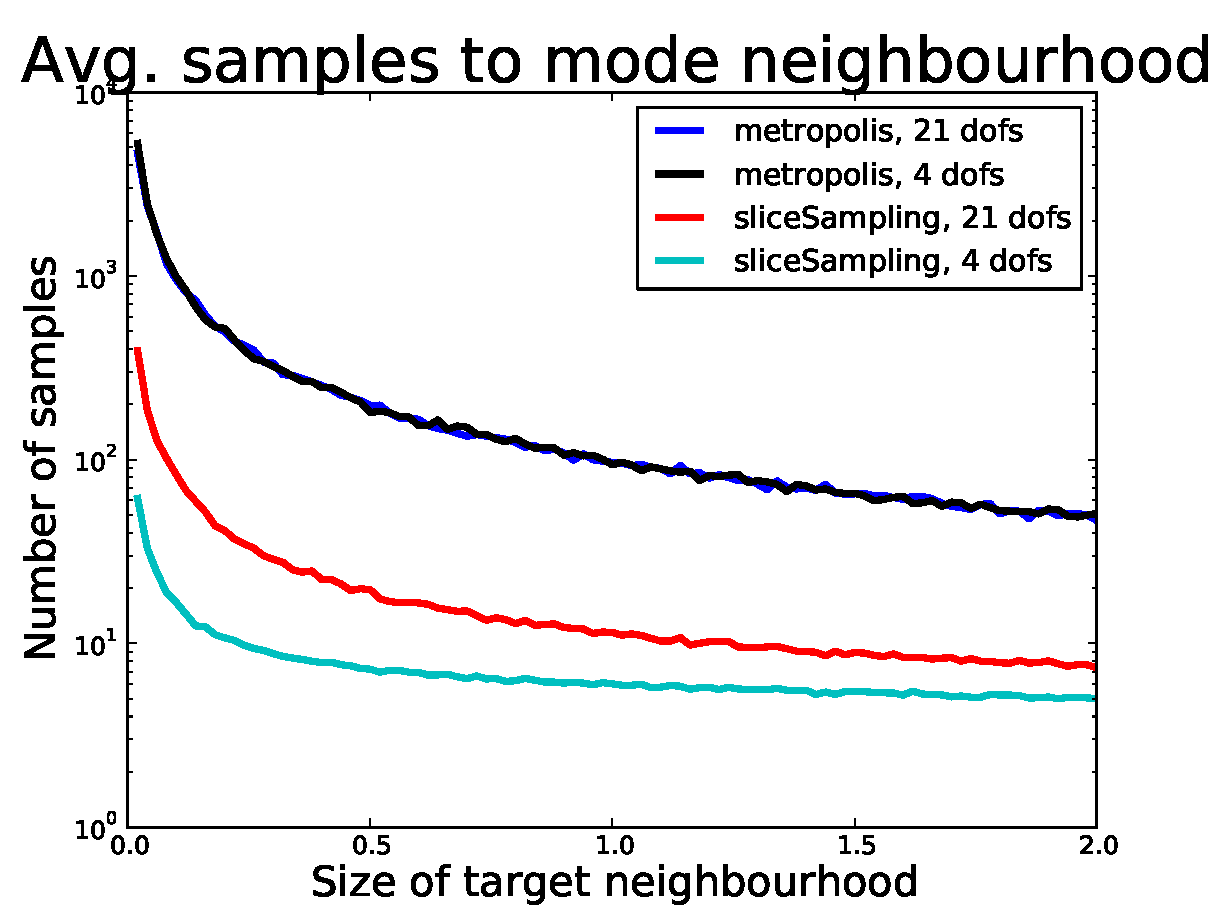
\includegraphics[width=0.8\textwidth]{SliceMetCustPerf}
    \caption{Burn-in time for local metropolis-hastings and slice sampling, on the two continuous Tdf models, as the target neighbourhood varies.}
    \label{fig:SliceMetCustPerf}
\end{figure}

However the performance of slice sampling does seem to vary with the shape of the likelihood. In Figure \ref{fig:sliceGaussLik} we investigate this behaviour by modeling the likelihood as a Gaussian and seeing how slice performs as we vary the Gaussian's properties.

\begin{figure}[h]
    \centering
    \begin{subfigure}[t]{0.48\textwidth}
      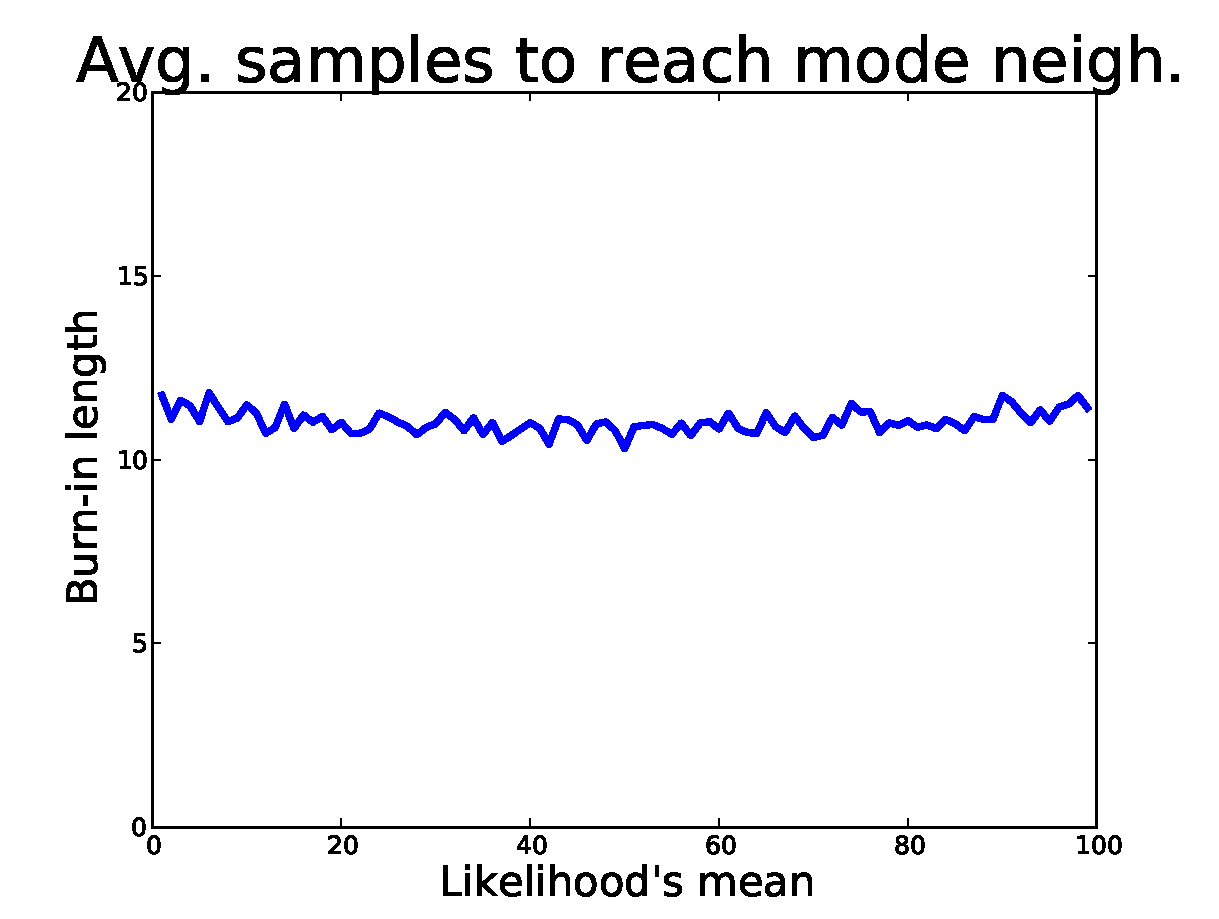
\includegraphics[width=\textwidth]{SliceSampsMean}
      \caption{Effect of likelihood mean}
    \end{subfigure}
    ~
    \begin{subfigure}[t]{0.48\textwidth}
      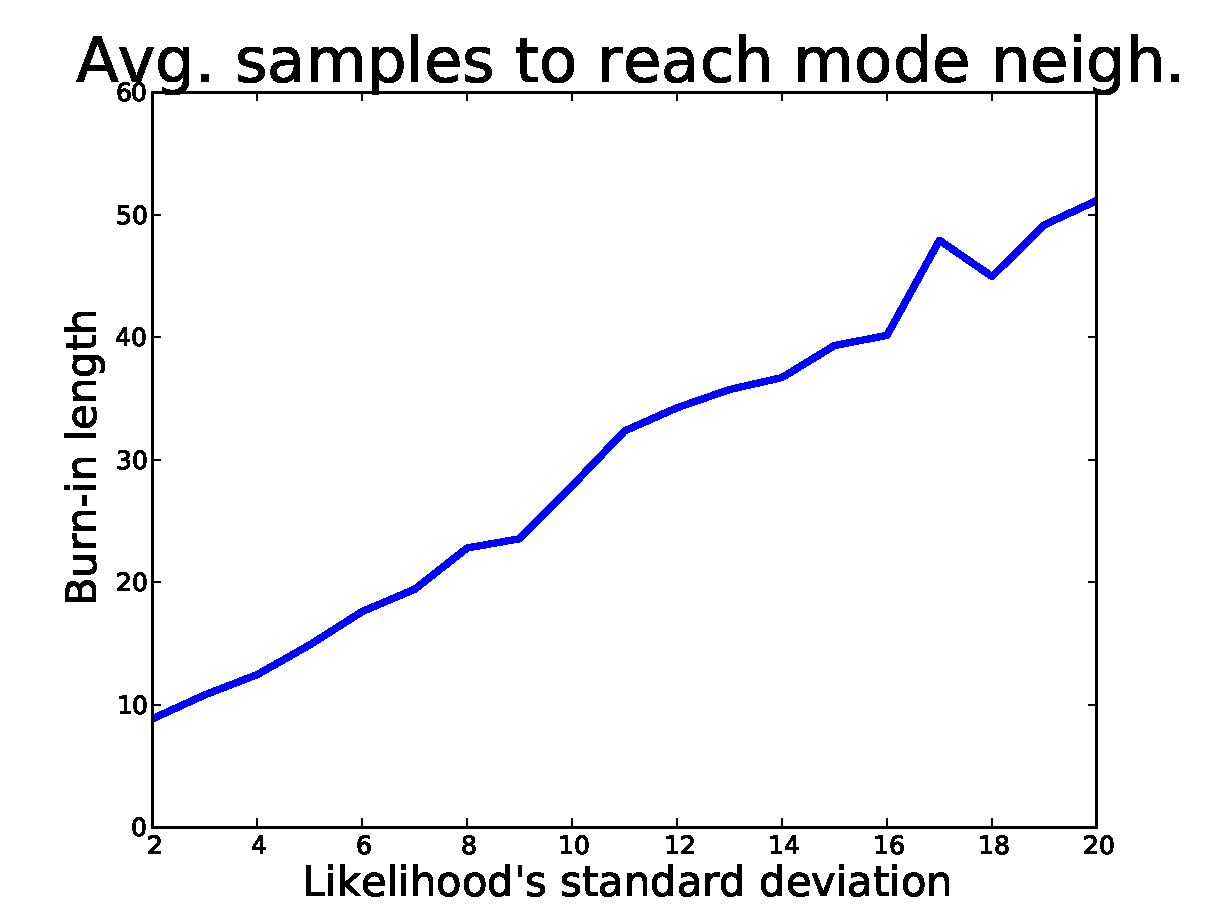
\includegraphics[width=\textwidth]{SliceSampsStd}
      \caption{Effect of likelihood standard deviation}
    \end{subfigure}
    \caption{Average burn-in time for slice sampling guided by a Gaussian likelihood of varying mean and standard deviation}
    \label{fig:sliceGaussLik}
\end{figure}

It seems that the placement of the likelihood in the interval doesn't affect performance, but the width of the distribution does. For reference, the Gaussian likelihoods with minimum and maximum standard deviations that we tested are shown in Figure \ref{fig:gaussStdDev}.

\begin{figure}[h]
    \centering
    \begin{subfigure}[t]{0.48\textwidth}
      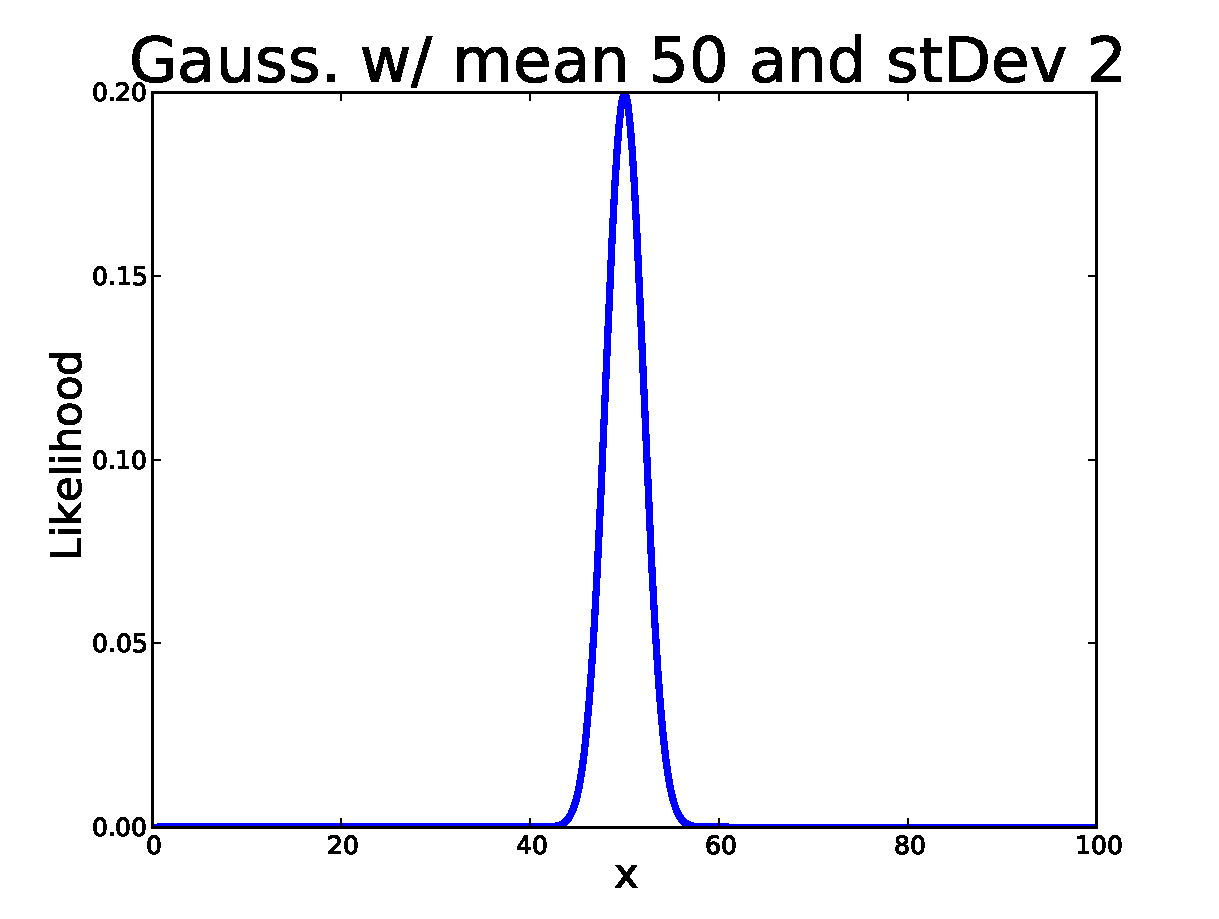
\includegraphics[width=\textwidth]{Gauss2}
    \end{subfigure}
    ~
    \begin{subfigure}[t]{0.48\textwidth}
      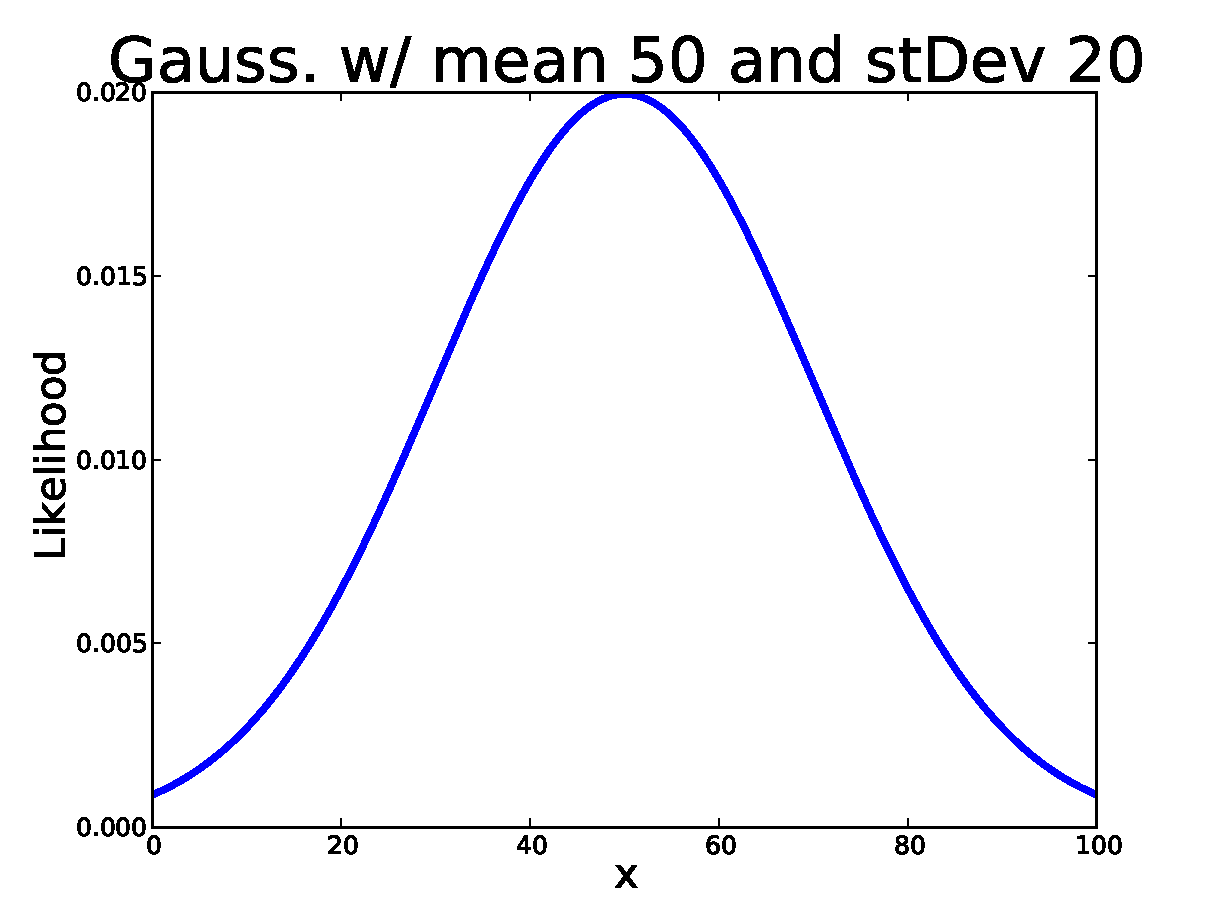
\includegraphics[width=\textwidth]{Gauss20}
    \end{subfigure}
    \caption{The smallest and largest Gaussian standard deviation considered in Figure \ref{fig:sliceGaussLik}}
    \label{fig:gaussStdDev}
\end{figure}

Next, we examine the mixing properties of local metropolis-hastings and slice sampling by considering the sample evolution (Figure \ref{fig:custSampEvol}), the sample autocorelation (Figure \ref{fig:custAutoCorr}) and the empirical distributions (Figure \ref{fig:custSampDist}) obtained by the two methods. For the obtained distributions to be comparable, we keep the number of log-likelihood computations performed by the two methods equal. This means that, while metropolis-hastings is allowed 10,000 samples, we only take 1962 from slice sampling (since, on this model, slice sampling averages just over 5 likelihood computations per extracted sample).

\begin{figure}[h]
    \centering
    \begin{subfigure}[t]{0.48\textwidth}
      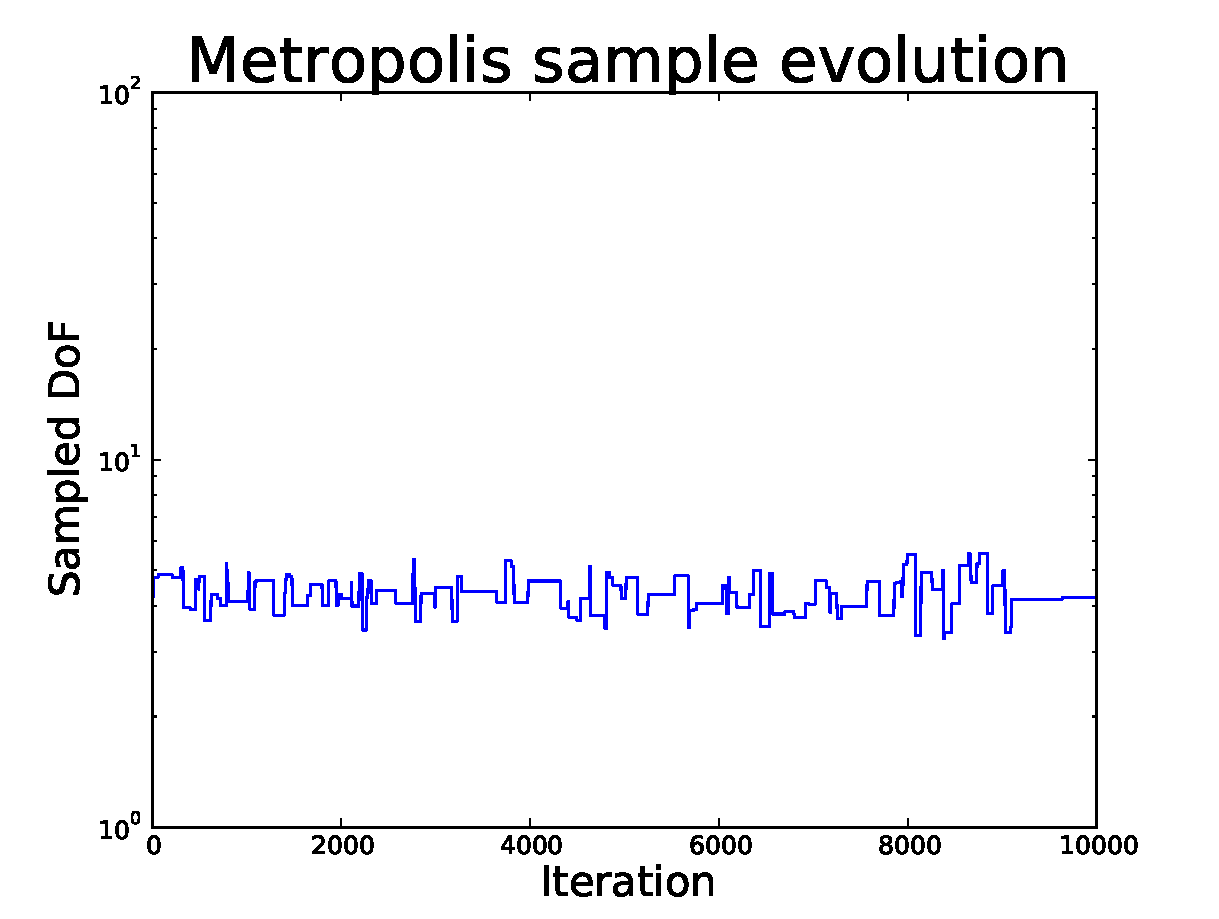
\includegraphics[width=\textwidth]{MetSampEvol}
    \end{subfigure}
    ~
    \begin{subfigure}[t]{0.48\textwidth}
      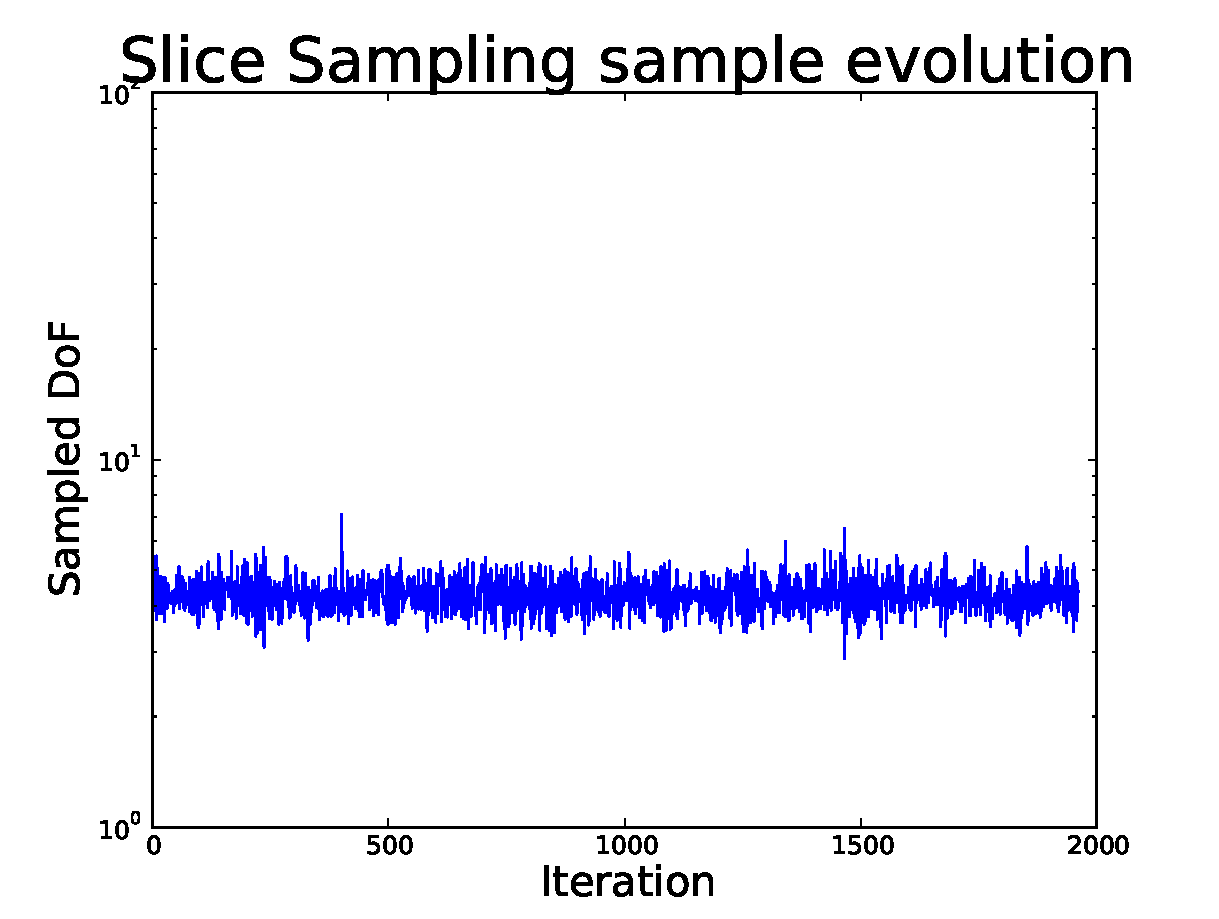
\includegraphics[width=\textwidth]{SliceSampEvol}
    \end{subfigure}
    \caption{Sample evolution of local metropolis and slice sampling on the Tdf continuous model}
    \label{fig:custSampEvol}
\end{figure}

\begin{figure}[h]
    \centering
    \begin{subfigure}[t]{0.48\textwidth}
      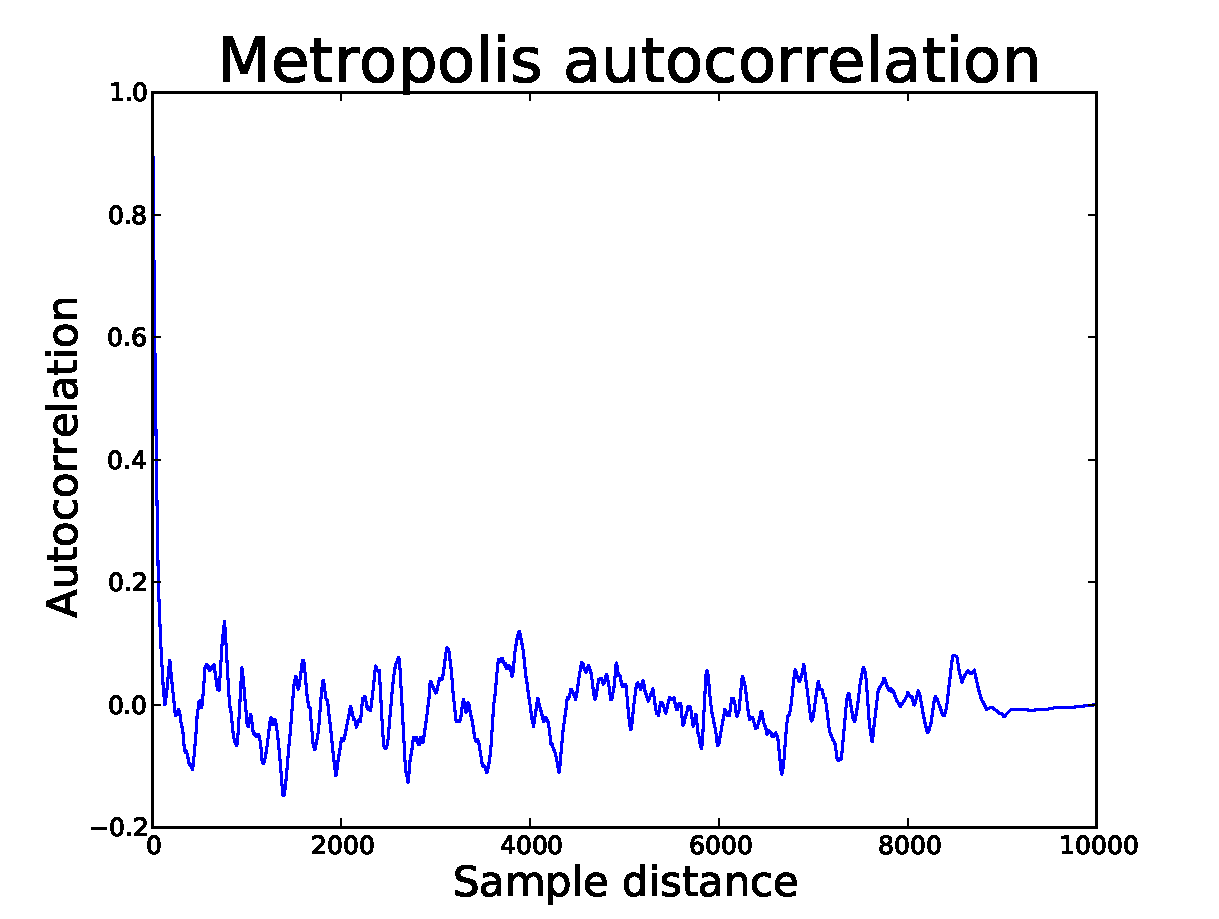
\includegraphics[width=\textwidth]{MetAutoCorr}
    \end{subfigure}
    ~
    \begin{subfigure}[t]{0.48\textwidth}
      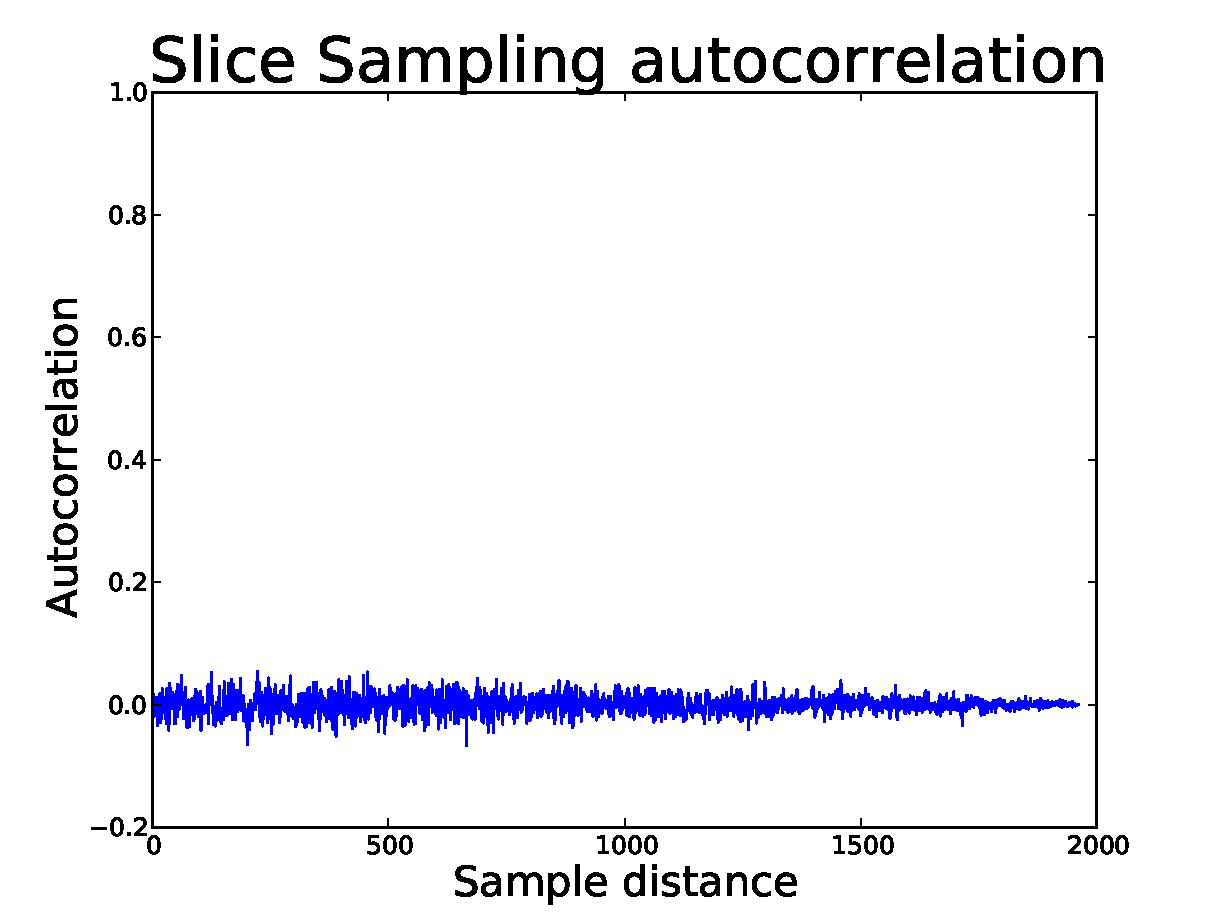
\includegraphics[width=\textwidth]{SliceAutoCorr}
    \end{subfigure}
    \caption{Sample autocorrelation of local metropolis and slice sampling on the Tdf continuous model}
    \label{fig:custAutoCorr}
\end{figure}

\begin{figure}[H]
    \centering
    \begin{subfigure}[t]{0.48\textwidth}
      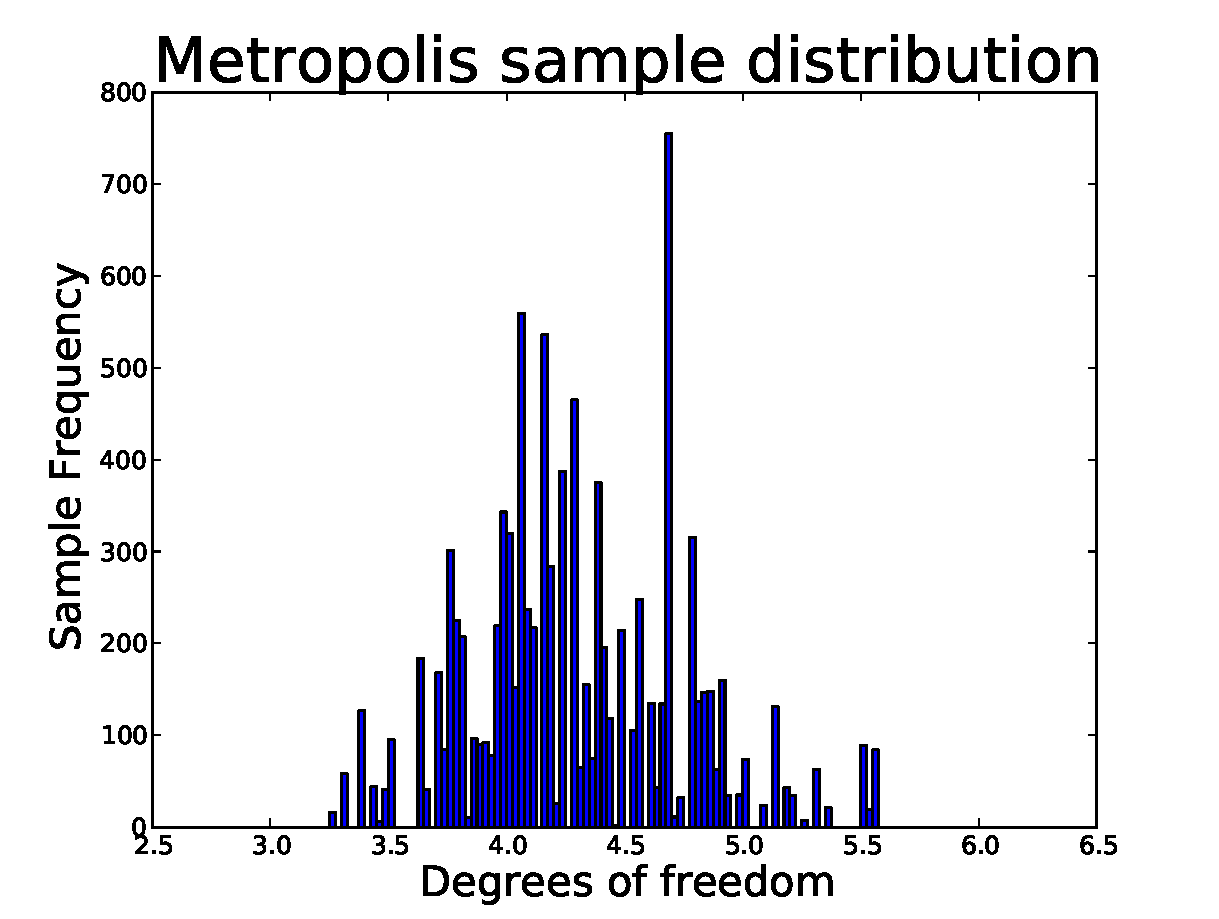
\includegraphics[width=\textwidth]{MetSampDist}
    \end{subfigure}
    ~
    \begin{subfigure}[t]{0.48\textwidth}
      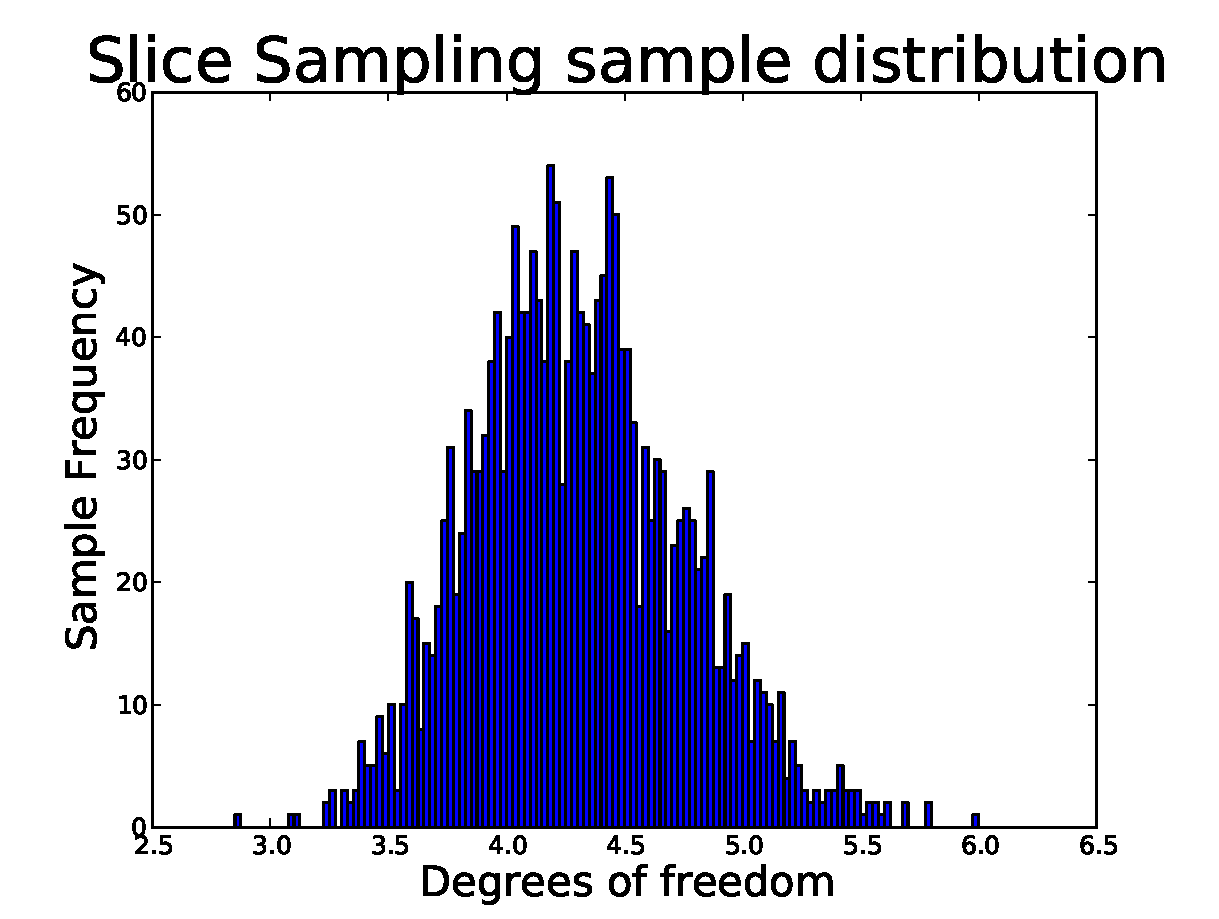
\includegraphics[width=\textwidth]{SliceSampDist}
    \end{subfigure}
    \caption{Empirical sample distribution of local metropolis and slice sampling on the Tdf continuous model}
    \label{fig:custSampDist}
\end{figure}

Based on these preliminary experiments slice sampling seems to confer a significant advantage over local metropolis when compared on the Tdf models.

\subsection{Generic, lightweight, slice sampling inference engine}

Since the custom slice sampling tests on the Tdf models gave promising results we next look at creating a generic slice sampling implementation that can run on arbitrary probabilistic programs. Our implementation, described in Section \ref{sect:StocPy}, follows the `Lightweight Implementations'' style of the PPLs \cite{wingate2011lightweight}. 

The slice sampling technique we use follows the basic ideas presented in Section \ref{sect:sliceBack}. The main points are:
\begin{itemize}

\item
sample a height $u$ uniformly from $[0, likelihood]$. Since we are working with log likelihoods that are too small to be exponentiated, we take the sample directly in logspace by sampling from the exponential corresponding to the log of u. Specifically, if our log likelihood is ll, then $u \sim -1 * (exp(1) + ll)$

\item
uniformly sample a random variable $cur$ to modify

\item
find values $xl$ and $xr$ smaller and larger than the current value $x$ of the random variable $cur$ such that the log likelihood under $xl$ and $xr$ is smaller than the height $u$. Search for these values in an exponential fashion, by doubling the last guess.

\item
uniformly sample a proposition for $cur$ from (uniform $xl$ $xr$). Resample until the log likelihood under the sample is larger than the height $u$.

\end{itemize}

The stochastic python metropolis implementation presented in Section \ref{sect:StocPy} runs the Tdf continuous model 2-2.5x slower than the Venture implementation. The metropolis implementation also runs about 6x faster than slice-sampling, per number of samples. As discussed above, the bollteneck is the number of trace likelihood calculations. The metropolis method calculated the log-likelihood exactly once for each sample while slice sampling will execute it a minimum of 3 times (one each for $xl$, $xr$ and $x$). In practice, due to the stepping out and the possible resampling of a variable, we average 6 log-likelihood calculations per sample, thus explaining the 6x slow-down.

This shows that, for the tdf model, tweaking the initial width and interval search strategies as to reduce the number of log-likelihood calculations will result in a further improvement of no more than 2x.

\subsubsection{Slice sampling on the Tdf model}
We first run the 3 methods (my stochastic python metropolis and slice sampling implementations and Venture) for 10 minutes. The resulting distributions are shown in Figure \ref{fig:tdfSampDists}.

\begin{figure}[h]
        \centering
        \begin{subfigure}[b]{0.31\textwidth}
                \centering
                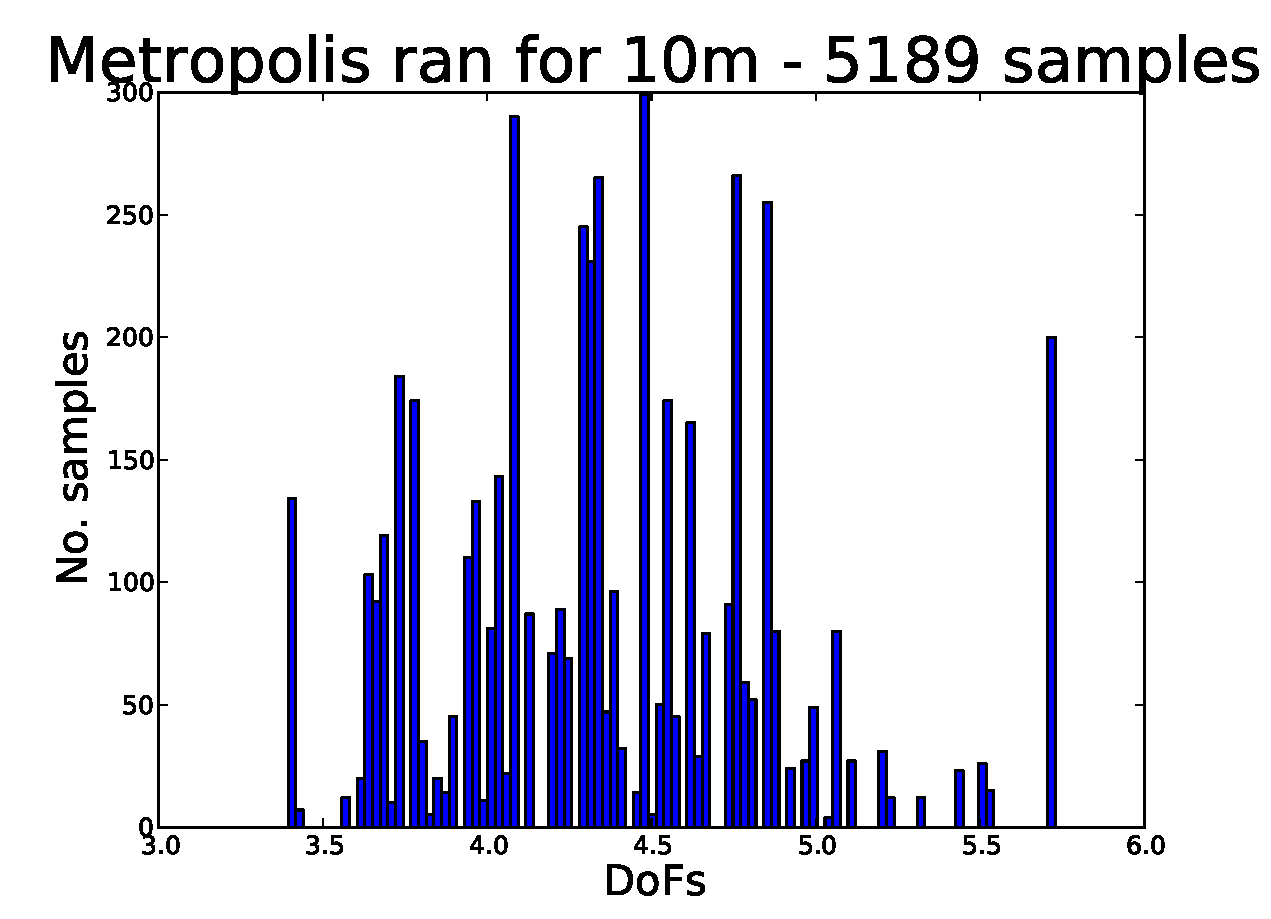
\includegraphics[width=\textwidth]{MetLISampDist}
        \end{subfigure}
        ~ 
        \begin{subfigure}[b]{0.31\textwidth}
                \centering
                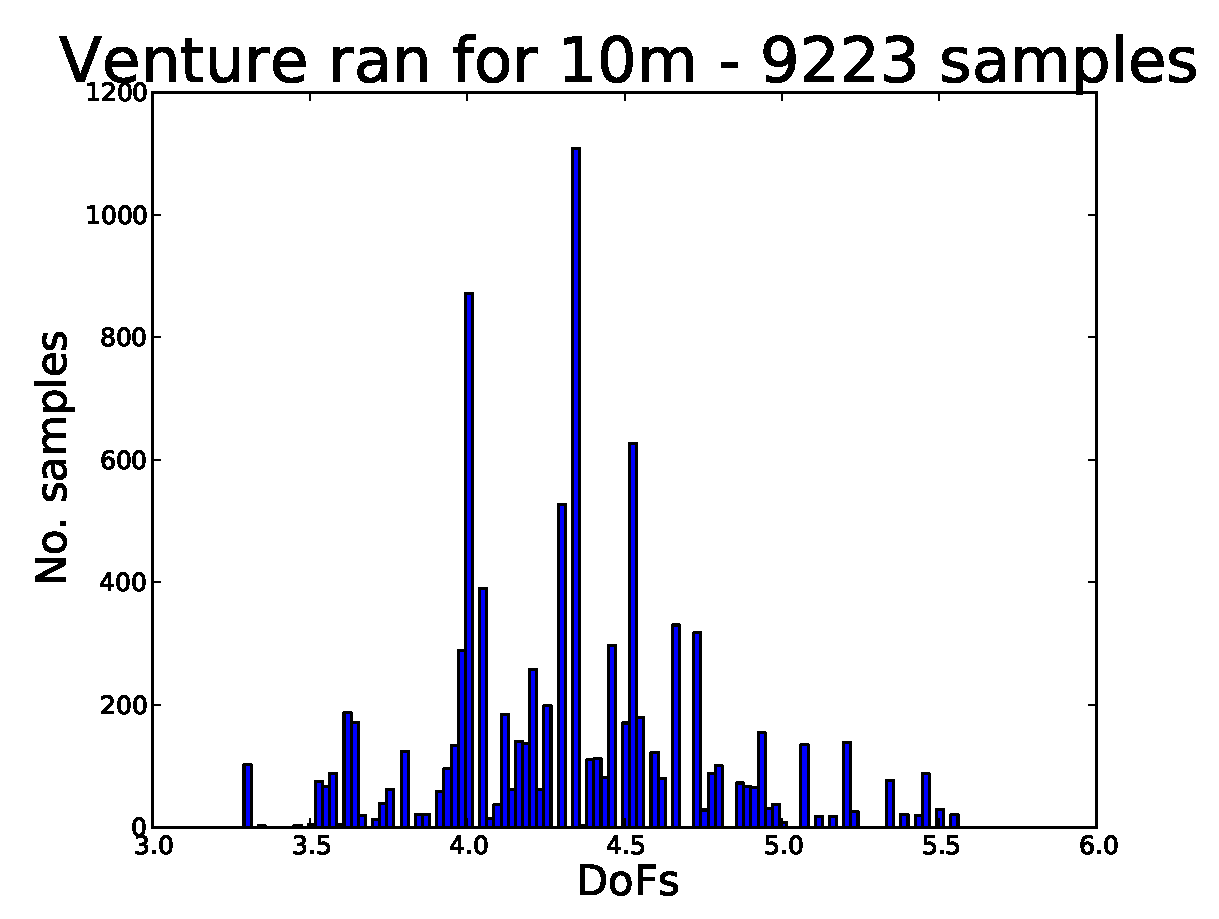
\includegraphics[width=\textwidth]{VentureLISampDist}
        \end{subfigure}
        ~ 
        \begin{subfigure}[b]{0.31\textwidth}
                \centering
                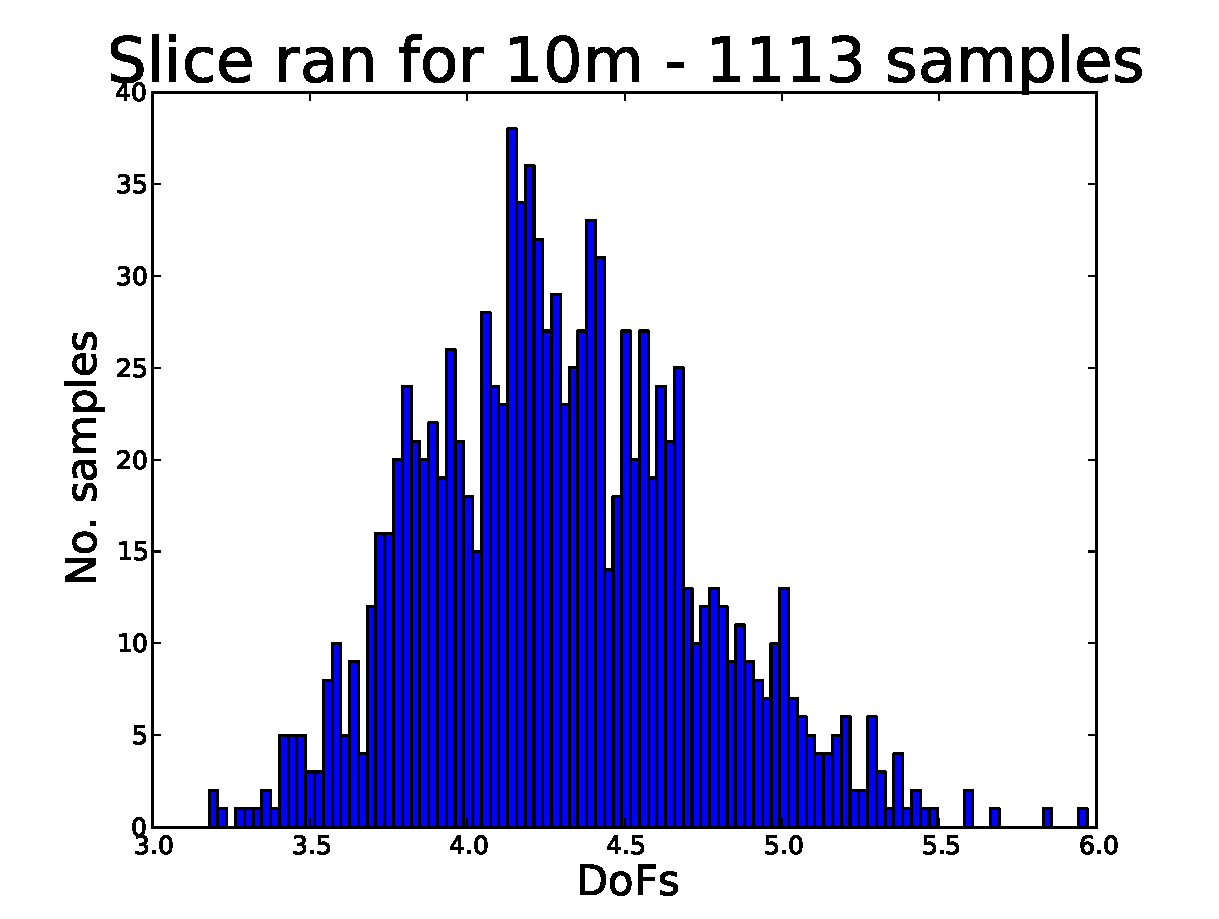
\includegraphics[width=\textwidth]{SliceLISampDist}
        \end{subfigure}
    \caption{Sample distribution from running Venture and stochastic python versions of metropolis and slice sampling for 10 minutes on the Tdf continuous model.}
    \label{fig:tdfSampDists}
\end{figure}

Visually, slice sampling appears to be doing the best job despite generating much fewer samples in 10 minutes than the other methods. In order to get a quantitative evaluation of the methods we can use the Kolmogorov-Smirnov statistic and plot a graph of the decreasing differences between the true cumulative distribution and the cumulative distributions inferred by the 3 methods. This experiment (see Figure \ref{fig:TdfSliceLIComp}) confirms our intuition and shows slice sampling significantly outperforming the other variants. 

\begin{figure}[h]
    \centering
    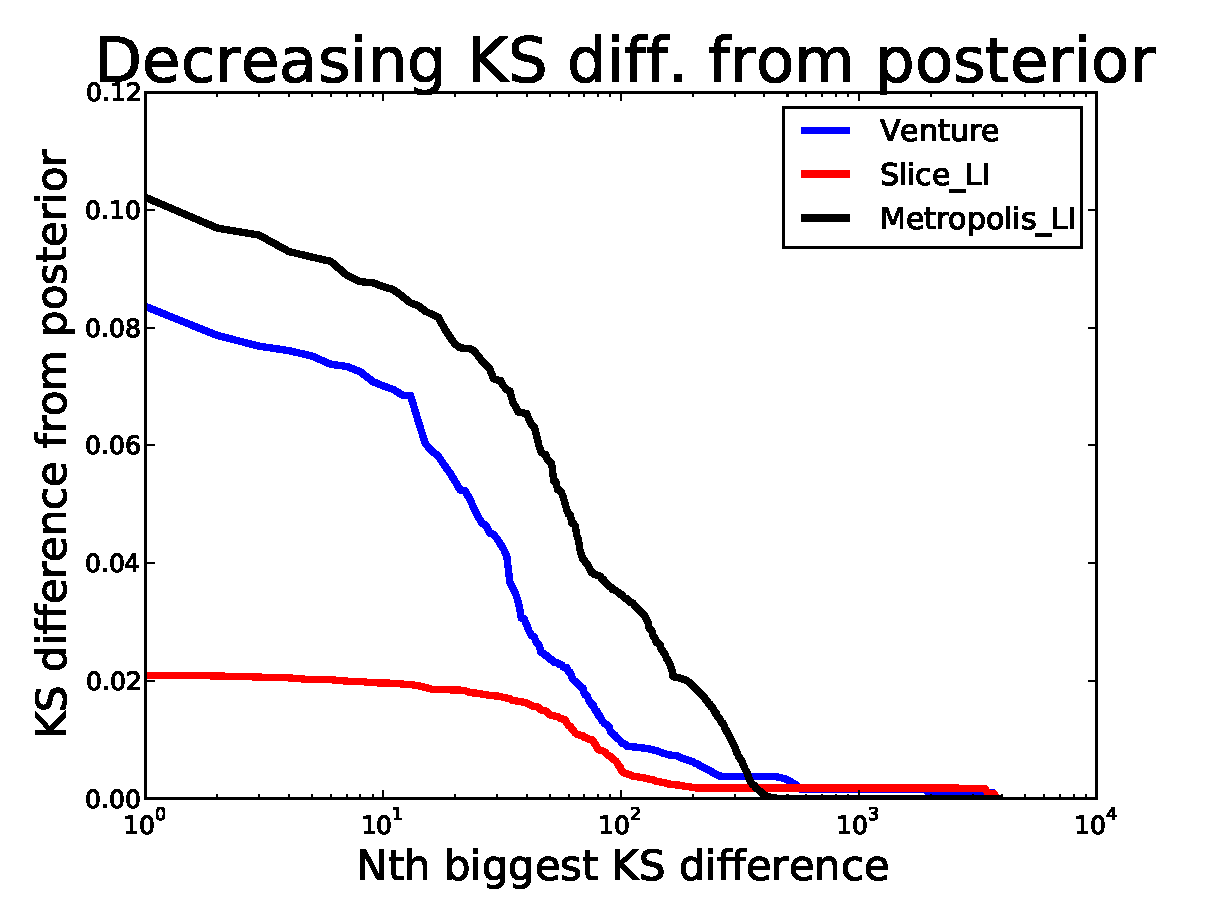
\includegraphics[width=0.8\textwidth]{TdfSliceLIComp}
    \caption{Comparison of Kolmogorov-Smirnov differences between true and inferred posteriors.}
    \label{fig:TdfSliceLIComp}
\end{figure}

\subsubsection{Slice sampling on gaussian mean inference models}
To further test the inference performance of metropolis and slice sampling I defined 3 models based on the problem of estimating the mean of a gaussian. The 3 models are and their posteriors are:

\noindent\begin{minipage}[t]{.32\textwidth}
\begin{flalign*}
  &NormalMean1: &
  \\ &\quad\quad m \sim N(0,1) &
  \\ &\quad\quad \text{observe }N(m,1) = 5 &
  \\ &\quad\quad \text{predict }m &
\end{flalign*}
\end{minipage}%
\begin{minipage}[t]{.32\textwidth}
\begin{flalign*}
  &NormalMean2: &
  \\ &\quad\quad m \sim N(0,1)
  \\ &\quad\quad v \sim invGamma(3,1)
  \\ &\quad\quad \text{observe }N(m,v) = 5
  \\ &\quad\quad \text{predict }m
\end{flalign*}
\end{minipage}%
\begin{minipage}[t]{.32\textwidth}
\begin{flalign*}
  &NormalMean3: &
  \\ &\quad\quad m \sim N(0,1)
  \\ &\quad\quad \text{if }m < 0
  \\ &\quad\quad\quad\quad v \sim invGamma(3,1)
  \\ &\quad\quad \text{else}
  \\ &\quad\quad\quad\quad v = 1/3
  \\ &\quad\quad \text{observe }N(m,v) = 5
  \\ &\quad\quad \text{predict }m
\end{flalign*}
\end{minipage}

\begin{figure}[h]
        \centering
        \begin{subfigure}[b]{0.31\textwidth}
                \centering
                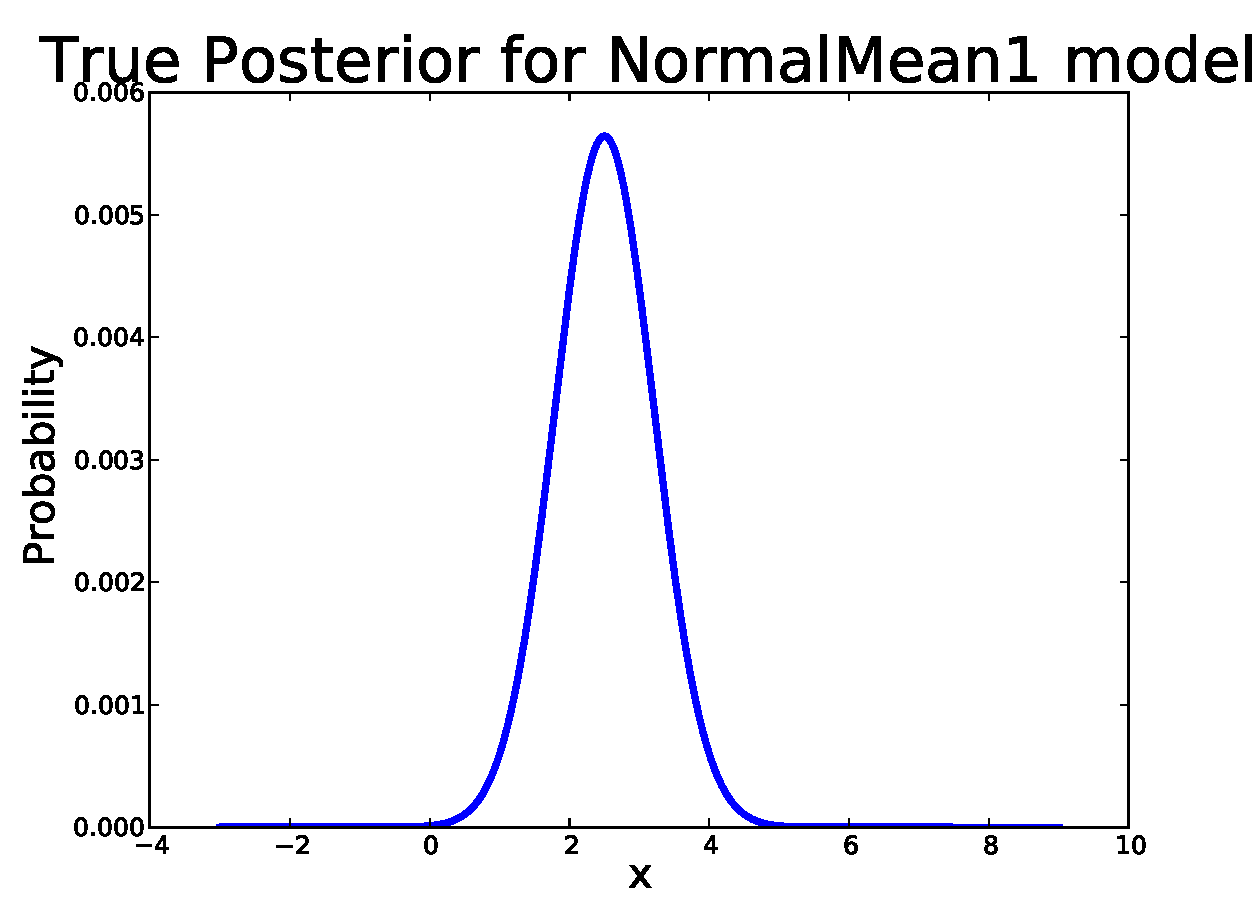
\includegraphics[width=\textwidth]{Normal1Post}
        \end{subfigure}
        ~ 
        \begin{subfigure}[b]{0.31\textwidth}
                \centering
                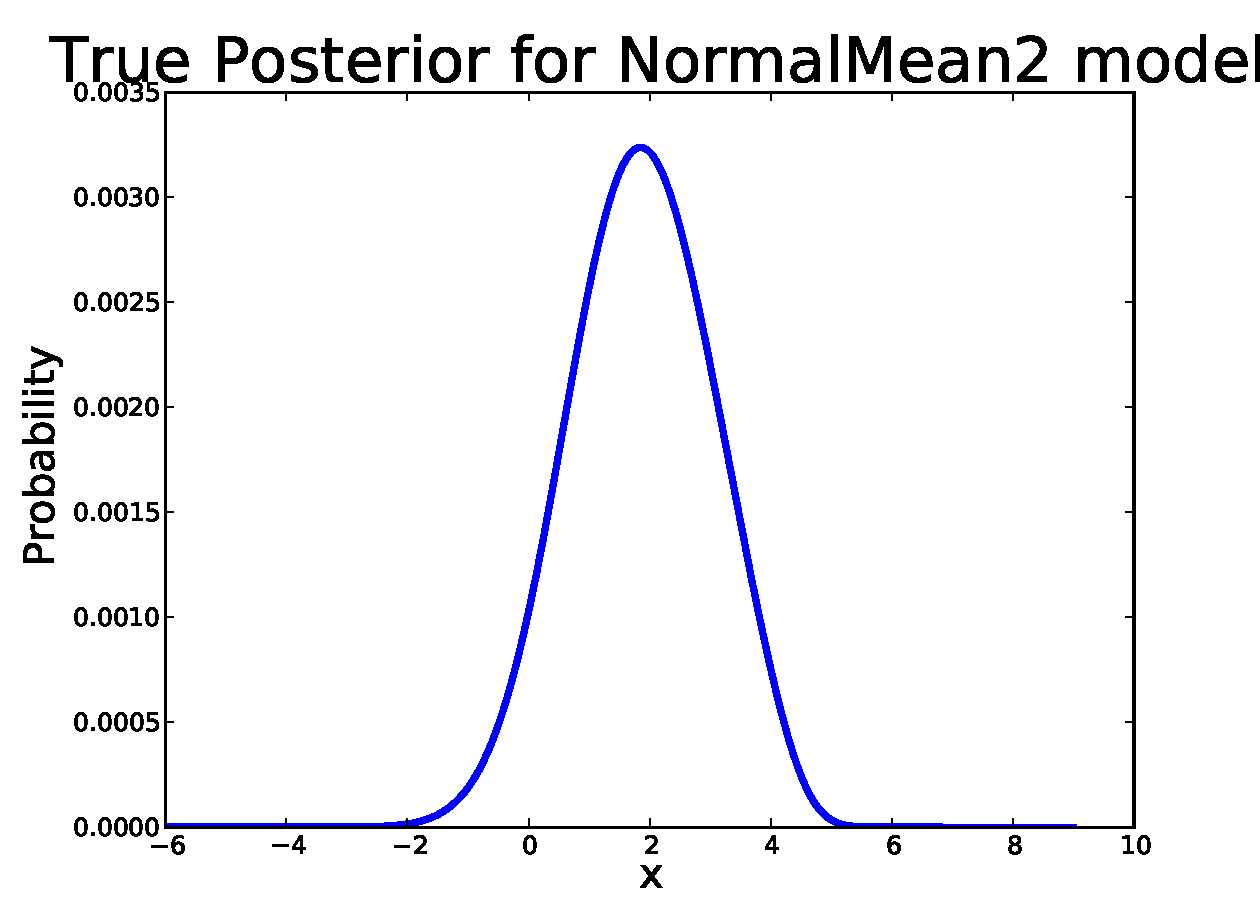
\includegraphics[width=\textwidth]{Normal2Post}
        \end{subfigure}
        ~ 
        \begin{subfigure}[b]{0.31\textwidth}
                \centering
                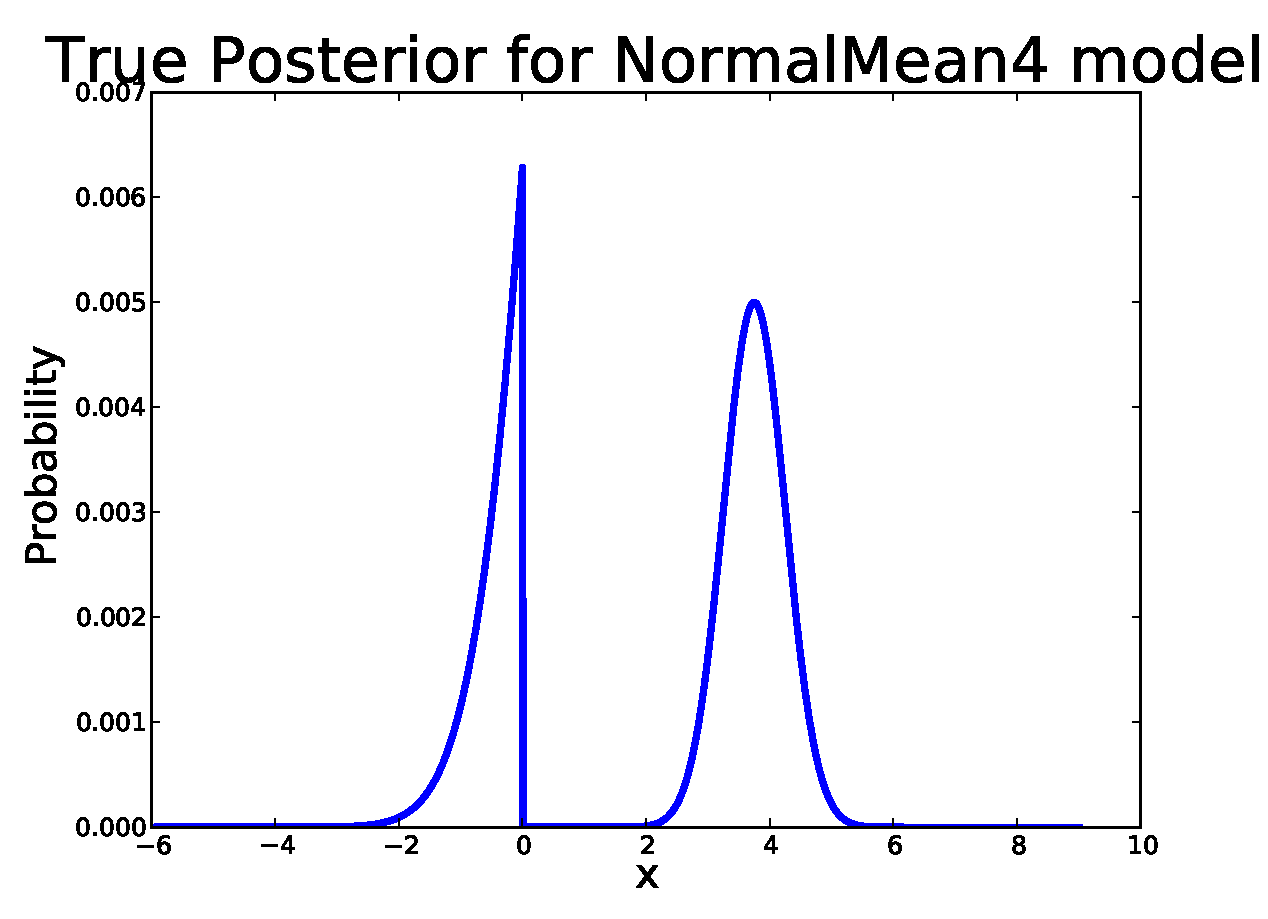
\includegraphics[width=\textwidth]{Normal4Post}
        \end{subfigure}
    \caption{Analytically derived posteriors of the NormalMean1, NormalMean2 and NormalMean3 models.}
    \label{fig:tdfSampDists}
\end{figure}

We now look at the performance of metropolis, slice sampling and different mixtures of slice sampling and metropolis (with different mixing proportions) over the 3 NormalMean models. The mixture methods work by flipping a biased coin before extracting each sample in order to decide which inference method to use. Since slice sampling cannot handle trans-dimensional jumps, we dissalow such jumps in the mixture algorithms. These algorithms are therefore reliant on metropolis to switch between program traces with different numbers of variables. 

To compare the inference engines, we extract samples untill a certain number of trace likelihood calculations are performed and then repeat this process 100 times, in order to generate independent sample runs (starting from different random seeds). Figure \ref{fig:normal1Perf} shows both the runs and the quartiles of the runs on the first model.

\begin{figure}[h]
        \centering
        \begin{subfigure}[b]{0.48\textwidth}
                \centering
                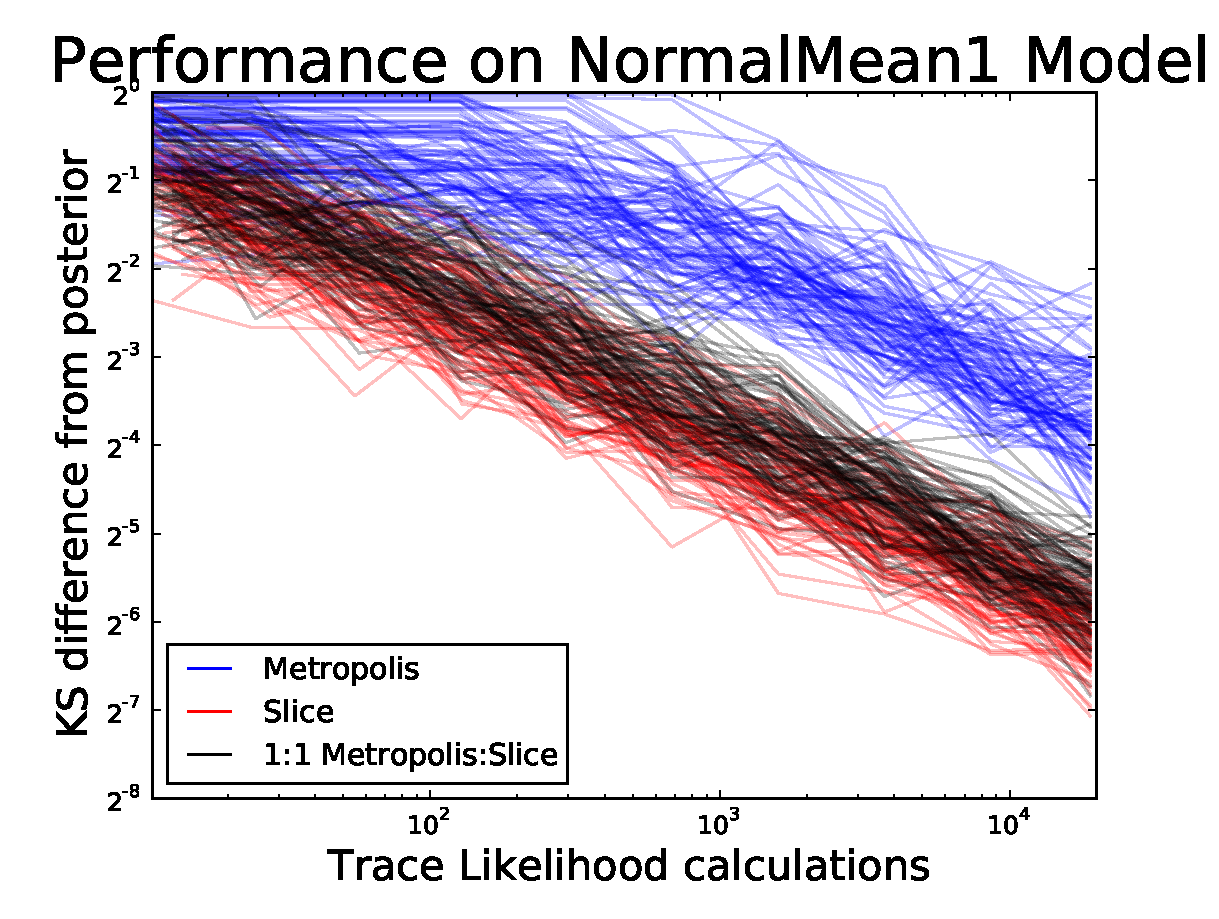
\includegraphics[width=\textwidth]{Normal1Runs}
        \end{subfigure}
        ~ 
        \begin{subfigure}[b]{0.48\textwidth}
                \centering
                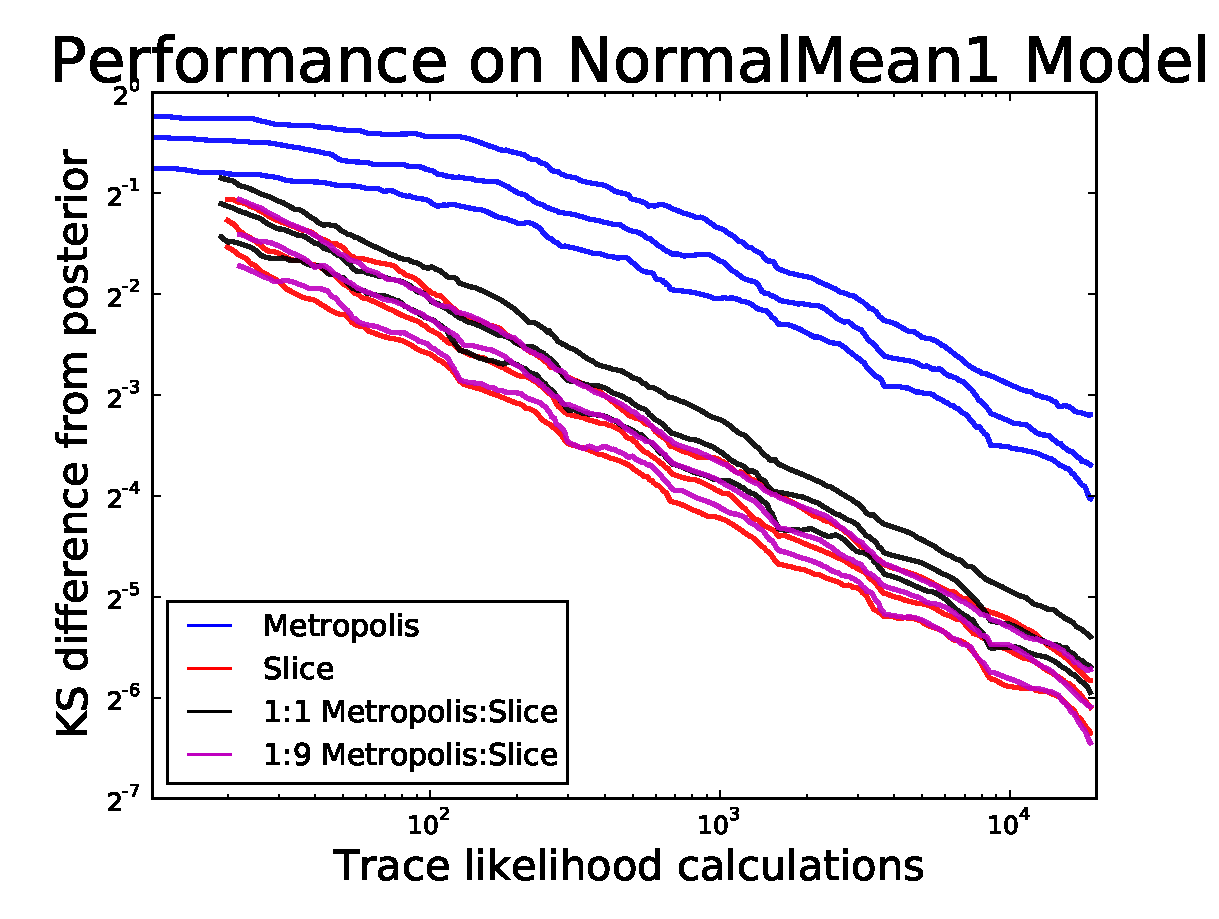
\includegraphics[width=\textwidth]{Normal1Quarts}
        \end{subfigure}
    \caption{Runs and quartiles generated by slice, metropolis and mixtures of metropolis and slice on the 1 dimensional NormalMean1 model.}
    \label{fig:normal1Perf}
\end{figure}

On the simple, 1d, model all variants of slice sampling clearly outperform metropolis. In the quartile graph we consider mixtures of metropolis and slice both with 10\% metropolis and with 50\% metropolis and find that the change doesn't have a significant impact on performance. This is likely because, if slice picks good samples, metropolis is likely to simply keep them unchanged (since it will tend to reject the proposal from the prior if they are worse).

\begin{figure}[h]
        \centering
        \begin{subfigure}[b]{0.48\textwidth}
                \centering
                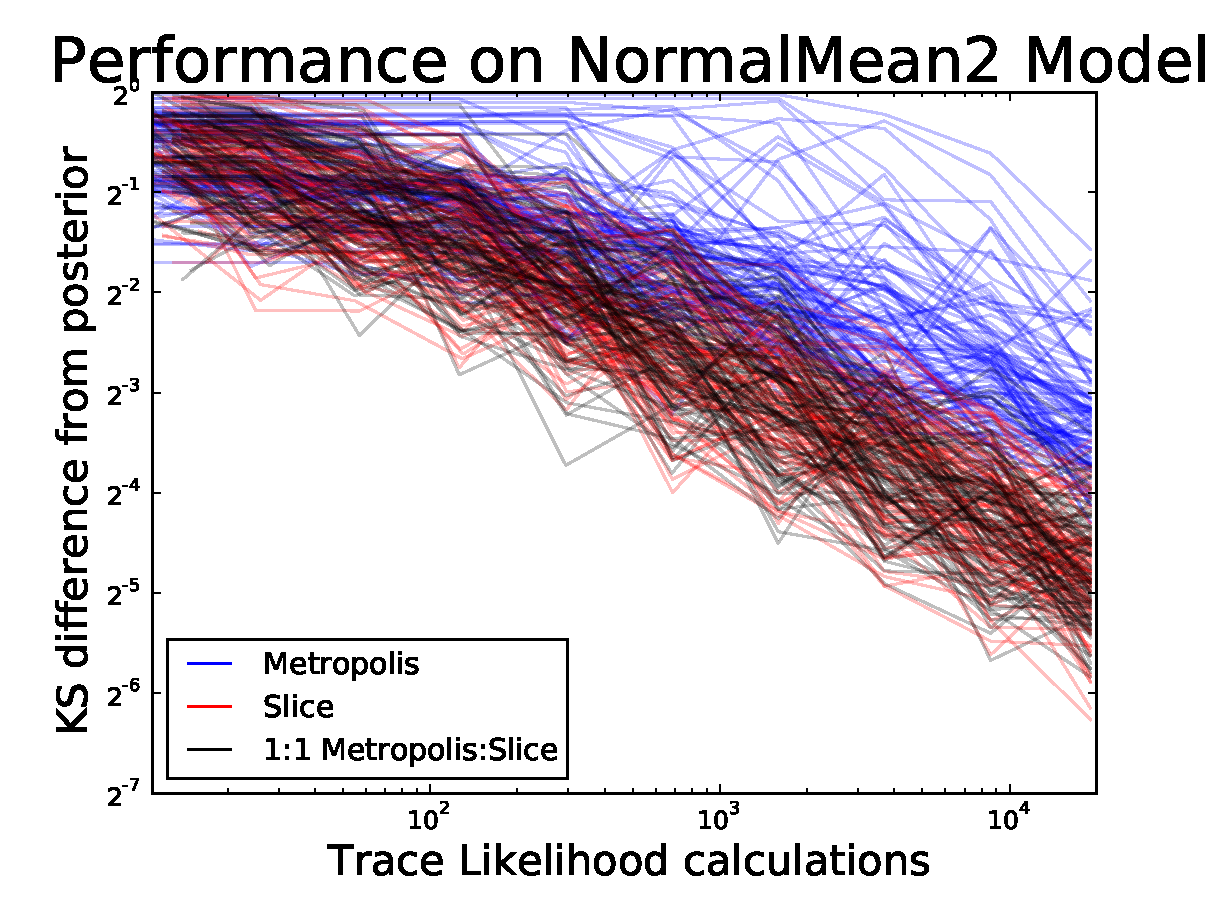
\includegraphics[width=\textwidth]{Normal2Runs}
        \end{subfigure}
        ~ 
        \begin{subfigure}[b]{0.48\textwidth}
                \centering
                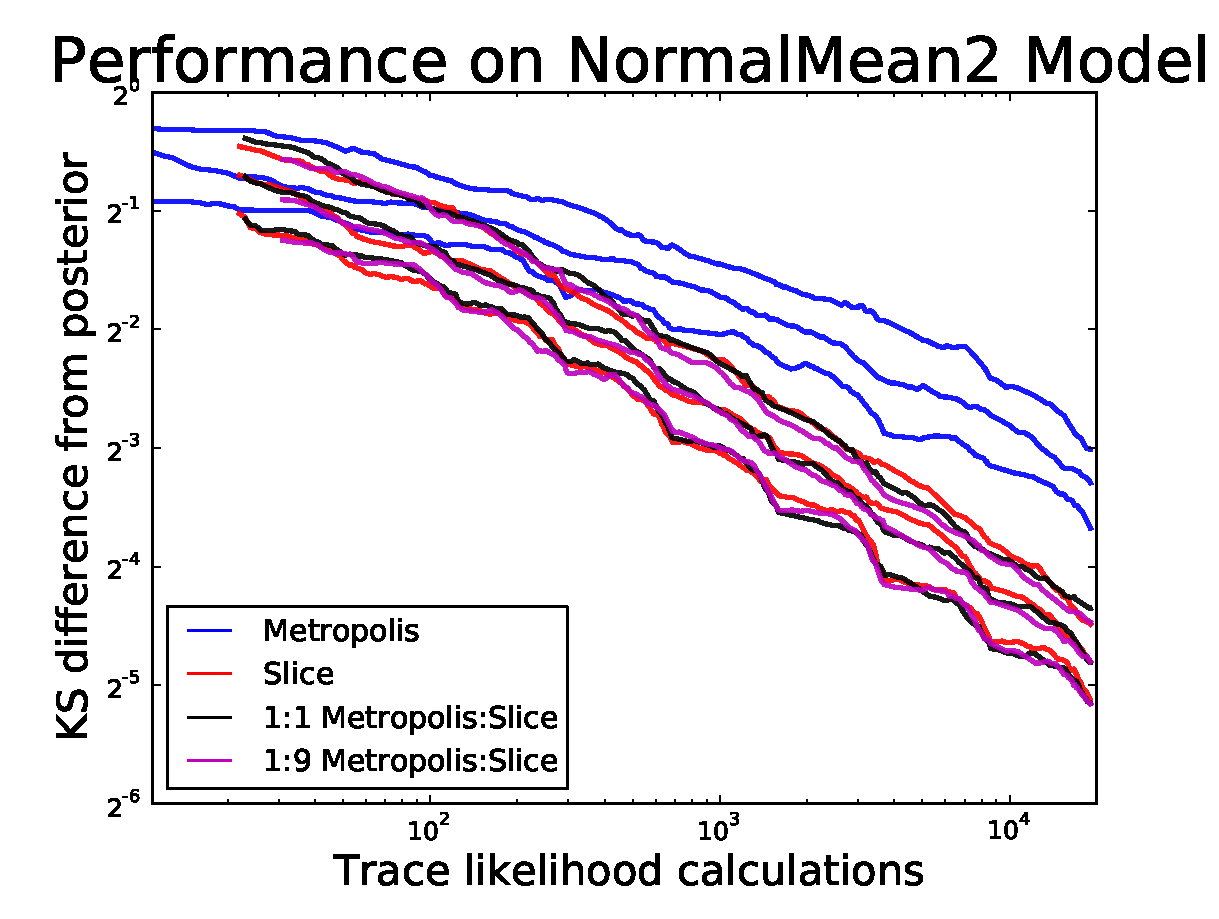
\includegraphics[width=\textwidth]{Normal2Quarts}
        \end{subfigure}
    \caption{Runs and quartiles generated by slice, metropolis and mixtures of metropolis and slice on the 2 dimensional NormalMean2 model.}
    \label{fig:normal2Perf}
\end{figure}

On the 2d model (see Figure \ref{fig:normal2Perf}), slice still clearly outperforms metropolis, though the gap is not as pronounced as for the 1d model. Further, as in the 1d model, the 3 different slice variants all get quite similar performance. Additionally, on this model, the fact that the slice mixtures get more samples per LL calculation translates into a slightly better performance for them than for the pure slice sampling method.

\begin{figure}[h]
        \centering
        \begin{subfigure}[b]{0.48\textwidth}
                \centering
                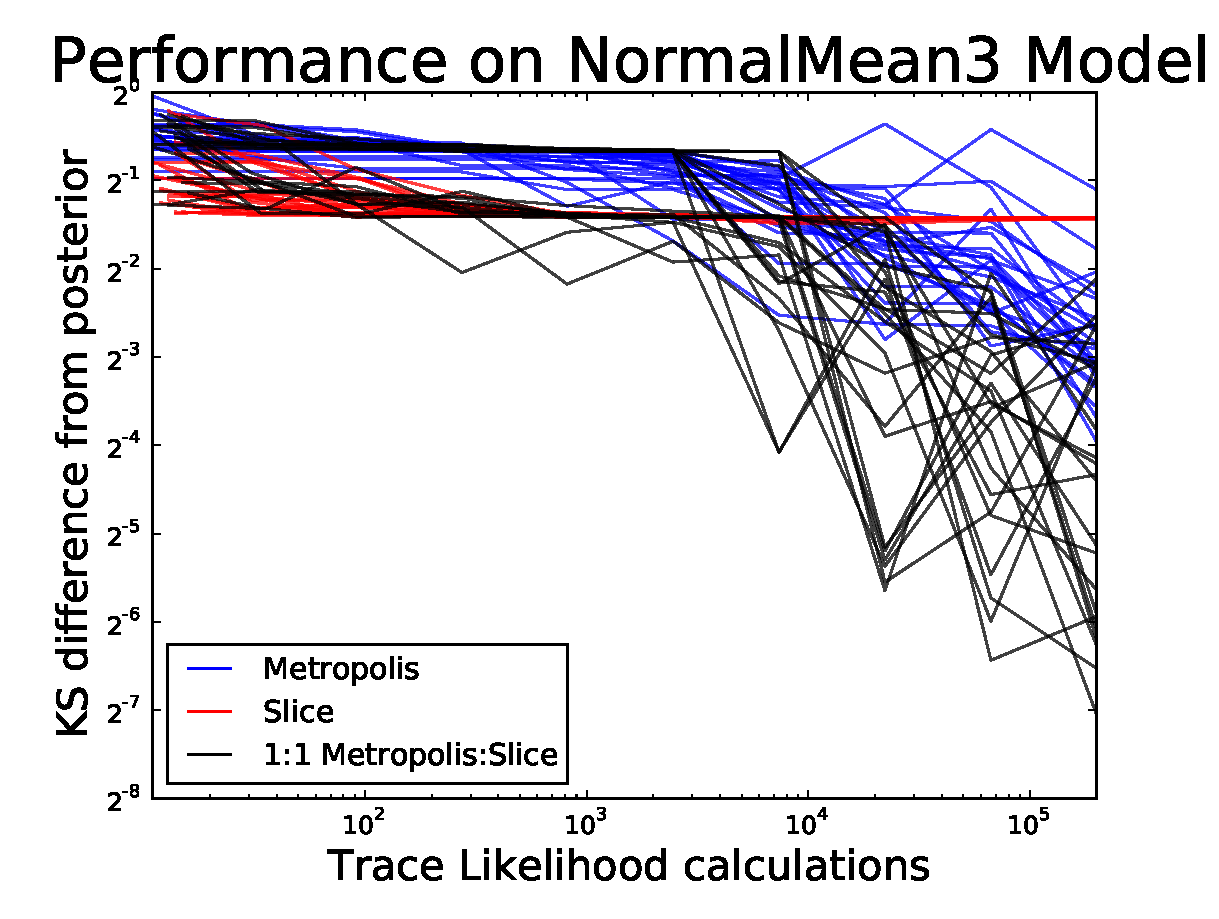
\includegraphics[width=\textwidth]{Normal4Runs}
        \end{subfigure}
        ~ 
        \begin{subfigure}[b]{0.48\textwidth}
                \centering
                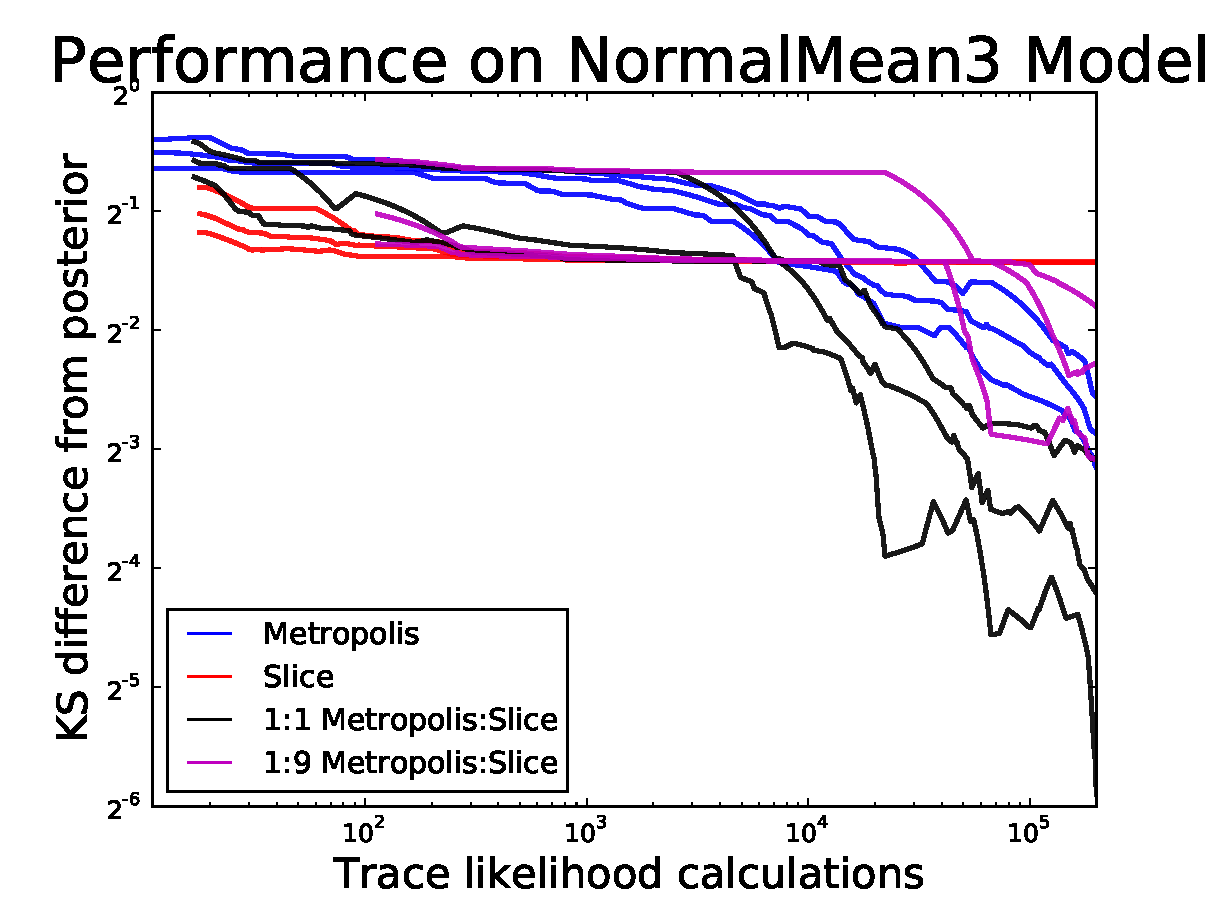
\includegraphics[width=\textwidth]{Normal4Quarts}
        \end{subfigure}
    \caption{Runs and quartiles generated by slice, metropolis and mixtures of metropolis and slice on the trans-dimensional NormalMean3 model.}
    \label{fig:normal4Perf}
\end{figure}

The third model, seen in Figure \ref{fig:normal4Perf}, reveals several things worth noting. First of all, pure slice sampling does very badly. This is because the simple slice sampling algorithm used in this example cannot handle trans-dimensional probabilistic models, such as NormalMean3. We will look closer at this problem in Section \ref{sect:tdSlice}. Further, on this model, we see the first significant performance gap between the different mixtures of slice and metropolis. Since slice sampling cannot handle trans-dimensional jumps, one of the main purposes of the metropolis steps in the mixture model is to switch between program traces with different dimensionality. In the case of the 1:9 Metropolis:Slice mixture, we see that this dimensionality switch happens quite rarely, and so the markov chain is stuck on bad samples for long runs. The 1:1 mixture of slice sampling and metropolis, however, manages to switch dimensionality sufficiently often and thus outperforms pure metropolis.

\subsubsection{Branching Model}
\label{sect:branching}
In order to further test the slice sampling inference engine we look at the Branching model considered in \cite{wood2014new}. This is also a trans-dimensional model, but this time operating on discrete data. The model specification we use is:

\begin{align*}
  Branching3:
  \\& pois1 \sim Poisson(4)
  \\&\text{if }pois1 > 4
  \\&\quad x = 6
  \\&else
  \\&\quad pois2 \sim Poisson(4)
  \\&\quad x = fib(3 * pois1) + pois2 \tag{$fib$ is the fibonacci function}
  \\&\text{observe }Poisson(x) = 6
  \\&\text{predict }pois1
\end{align*}

In order to test the convergence rate of the inference engines we must first analytically derive the true posterior for this model. This is given, up to values of 20 in Figure \ref{fig:BranchPost}.

\begin{figure}[h]
    \centering
    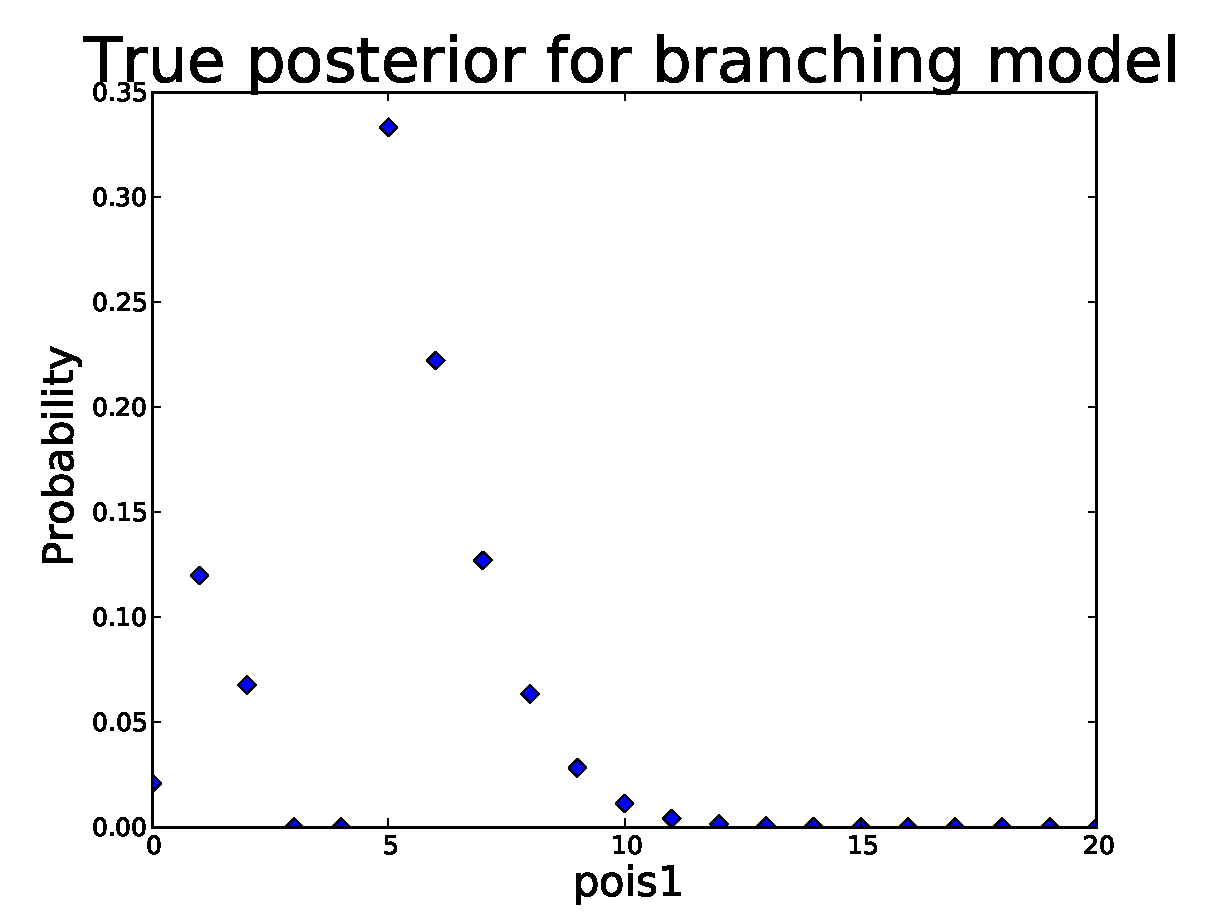
\includegraphics[width=0.8\textwidth]{BranchPost}
    \caption{True posterior for the Branching Model}
    \label{fig:BranchPost}
\end{figure}

In order to evaluate the engines, we use each to generate 100 independent sample runs, all performing an equal number of trace likelihood calculations. In Figure \ref{fig:branchPerf}, we plot the evolution of the KL divergences between the empirical and the true posterior as the number of trace likelihood calculations increase.

\begin{figure}[h]
        \centering
        \begin{subfigure}[b]{0.48\textwidth}
                \centering
                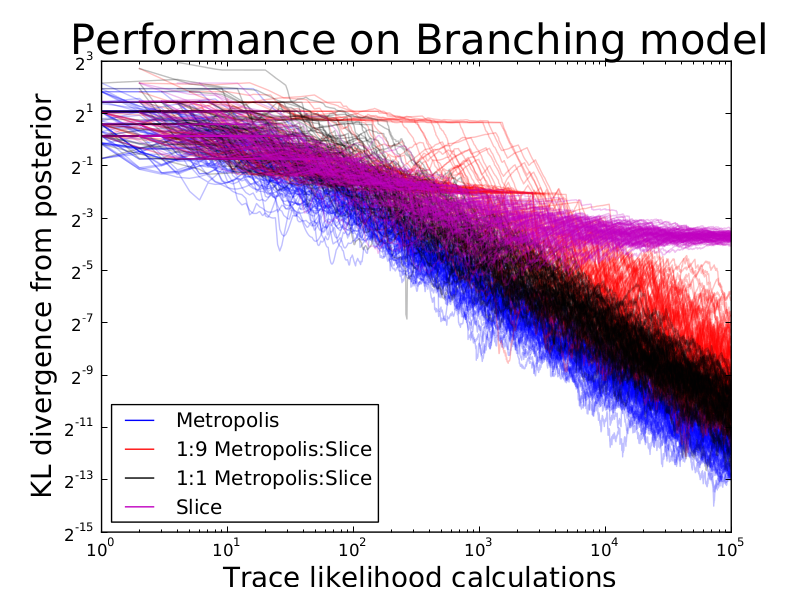
\includegraphics[width=\textwidth]{BranchRuns}
        \end{subfigure}
        ~ 
        \begin{subfigure}[b]{0.48\textwidth}
                \centering
                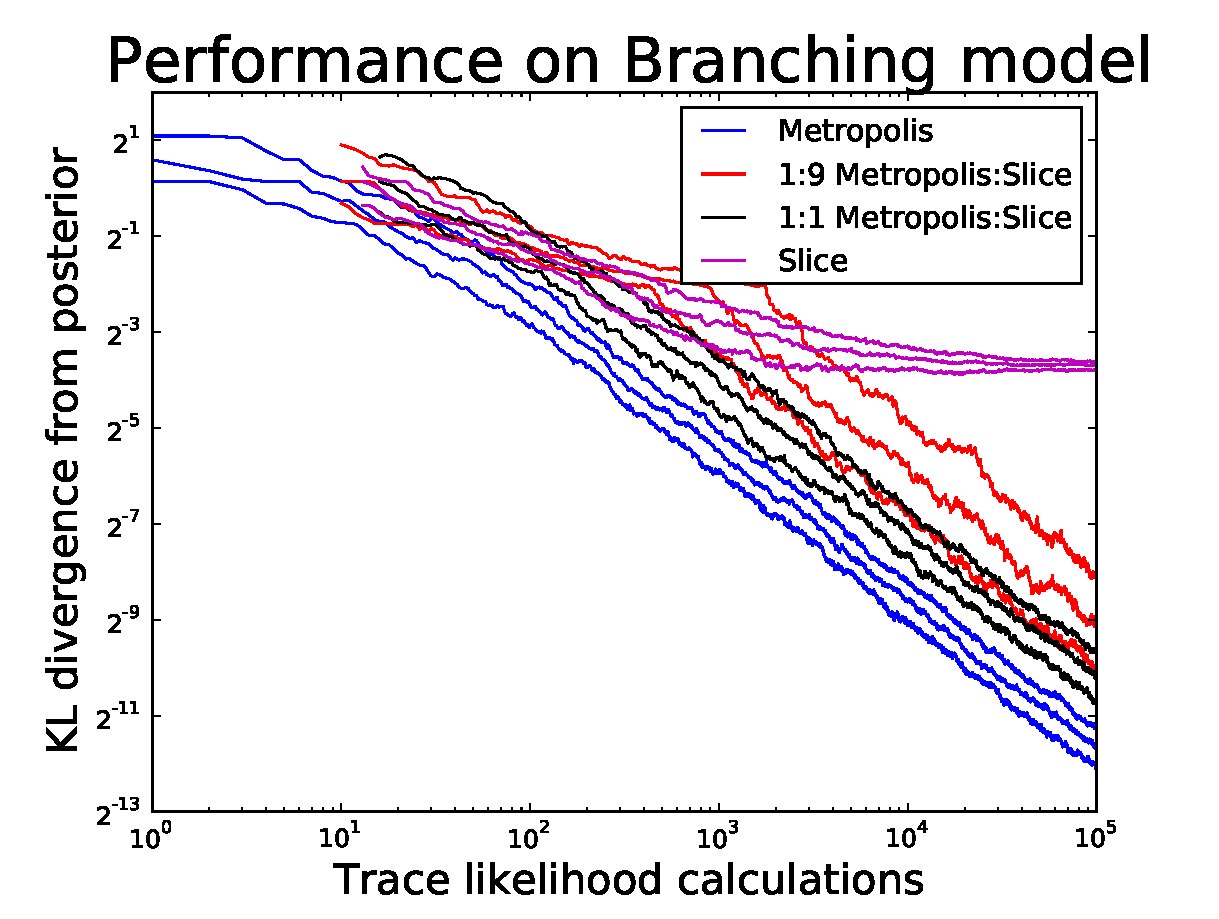
\includegraphics[width=\textwidth]{BranchQuarts}
        \end{subfigure}
    \caption{Runs and quartiles generated by slice, metropolis and mixtures of metropolis and slice on the Branching model.}
    \label{fig:branchPerf}
\end{figure}

As for the previous trans-dimensional model (NormalMode3), we see that the slice inference does not converge to the correct distribution since it cannot properly handle trans-dimensional jumps. The Metropolis:Slice mixtures do converge correctly but, on this model, are less efficient than the local Metropolis-Hastings.

One thing worth noting on this model, is that slice sampling proposes some values of pois1 that are extremely unlikely (such as 60). The reason it proposes these values is that it picks a slice height based on the trace log-likelihood which in this model can be extremely low due to the distribution of the conditioned upon variable (x). In the Branching model, likely values of the 2 random variables (based on their priors) can result in very unlikely program traces and these traces can then result in accepting very unlikely values of our 2 random variables, since the acceptance criterion is simply that the proposed trace have likelihood higher than a number drawn uniformly from [0, oldTraceLL].

However, we would expect this behaviour to only occur at the begining of a run, so the 1000 trace likelihood calculations burn-in period we are using should mitigate any influence this factor may have.

It's unclear why slice does worse on this model than on the NormalMean3 one, especially as the model distributions don't seem to affect the proposal efficiency, with both models averaging about 1 sample for 5 LL calculations.

It is informative to look at a per sample comparison of metropolis and slice sampling (see Figure \ref{fig:branchPerfSamps}), in addition to the previous per trace likelihood comparison (even though slice does ``more work'' to generate a sample than metropolis). In this plot we can see that the samples generated by 1:1 Metropolis:Slice are actually slightly better than the pure metropolis ones. However the difference is not large enough to make up for the extra trace likelihood calculations that slice sampling must perform. We can also notice that the slice sampling mixtures experience a larger variance in performance than the pure metropolis method. This may be due to the fact that we are relying on only the metropolis generated samples to randomly switch between the 2 modes in the posterior.

\begin{figure}[h]
        \centering
        \begin{subfigure}[b]{0.48\textwidth}
                \centering
                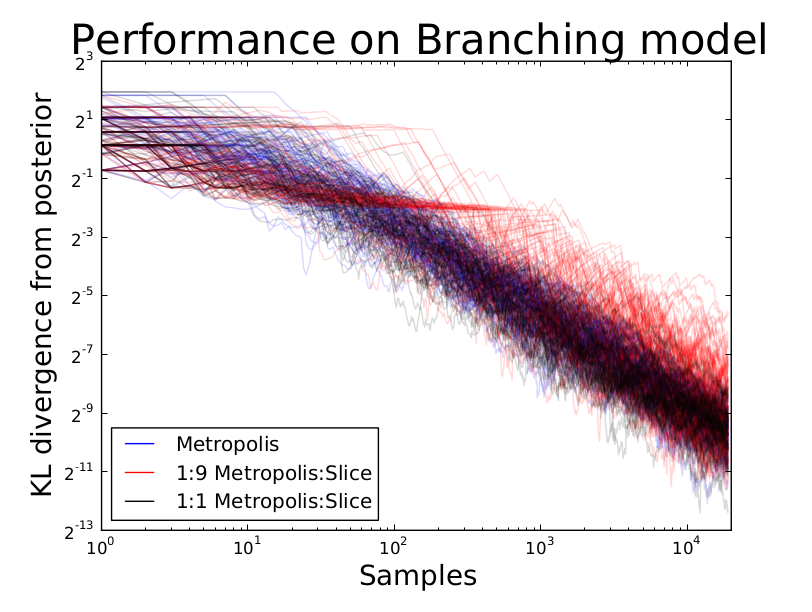
\includegraphics[width=\textwidth]{BranchRunsSamps}
        \end{subfigure}
        ~ 
        \begin{subfigure}[b]{0.48\textwidth}
                \centering
                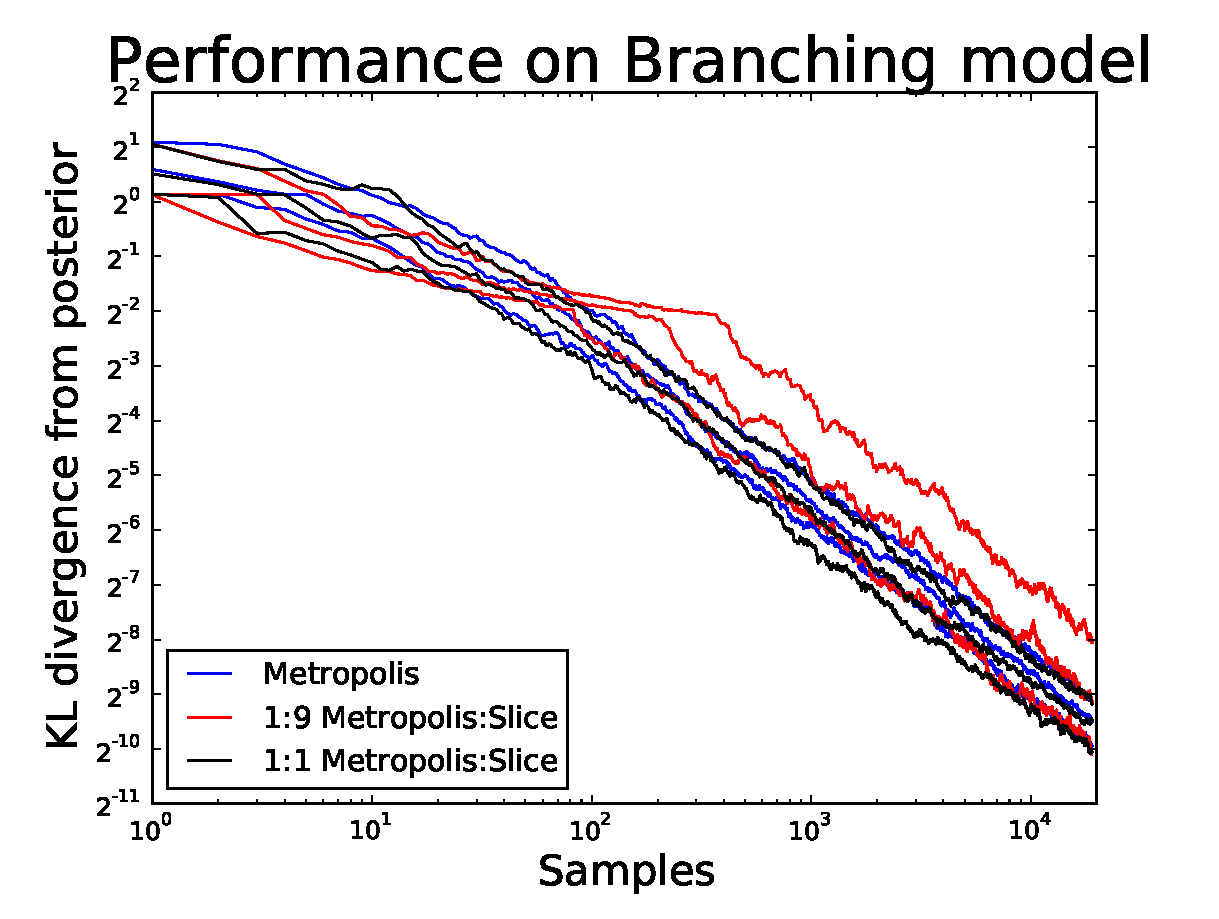
\includegraphics[width=\textwidth]{BranchQuartsSamps}
        \end{subfigure}
    \caption{Runs and quartiles generated by slice, metropolis and mixtures of metropolis and slice on the Branching model.}
    \label{fig:branchPerfSamps}
\end{figure}

\subsubsection{Trans-dimensional slice sampling}
\label{sect:tdSlice}
An interesting research question is whether (and how) it might be possible to modify the slice sampling algorithm so that it can correctly perform inference on probabilistic programs with varying numbers of dimensions.

As a pre-requisite to approaching this question, it is usefull to investigate what is going wrong when trying to perform inference on the Branching and NormalMean3 trans-dimensional models. On the Branching model investigated in Section \ref{sect:branching}, we see that the model has 2 random variables whose values determine the distribution of a 3rd variable which we condition on. This model is trans-dimensional since on different traces either one or both of the 2 variables will be sampled.

Re-writing the model so that both variables are always sampled, even if one of them is unused, leaves the posterior invariant. Therefore one method to correctly perform inference in a trans-dimensional model is to always sample all the variables that might ever be used in any trace. This approach will however be extremely inneficient in large models and is not a viable general solution. In Figure \ref{fig:branchTraceLik} we use this trick to see what the space of possible trace likelihoods looks like. Integrating out the pois2 variable from the above trace likelihood space results in the correct posterior distribution, shown in Figure \ref{fig:branchPost}).

\begin{figure}[h]
        \centering
        \begin{subfigure}[b]{0.48\textwidth}
                \centering
                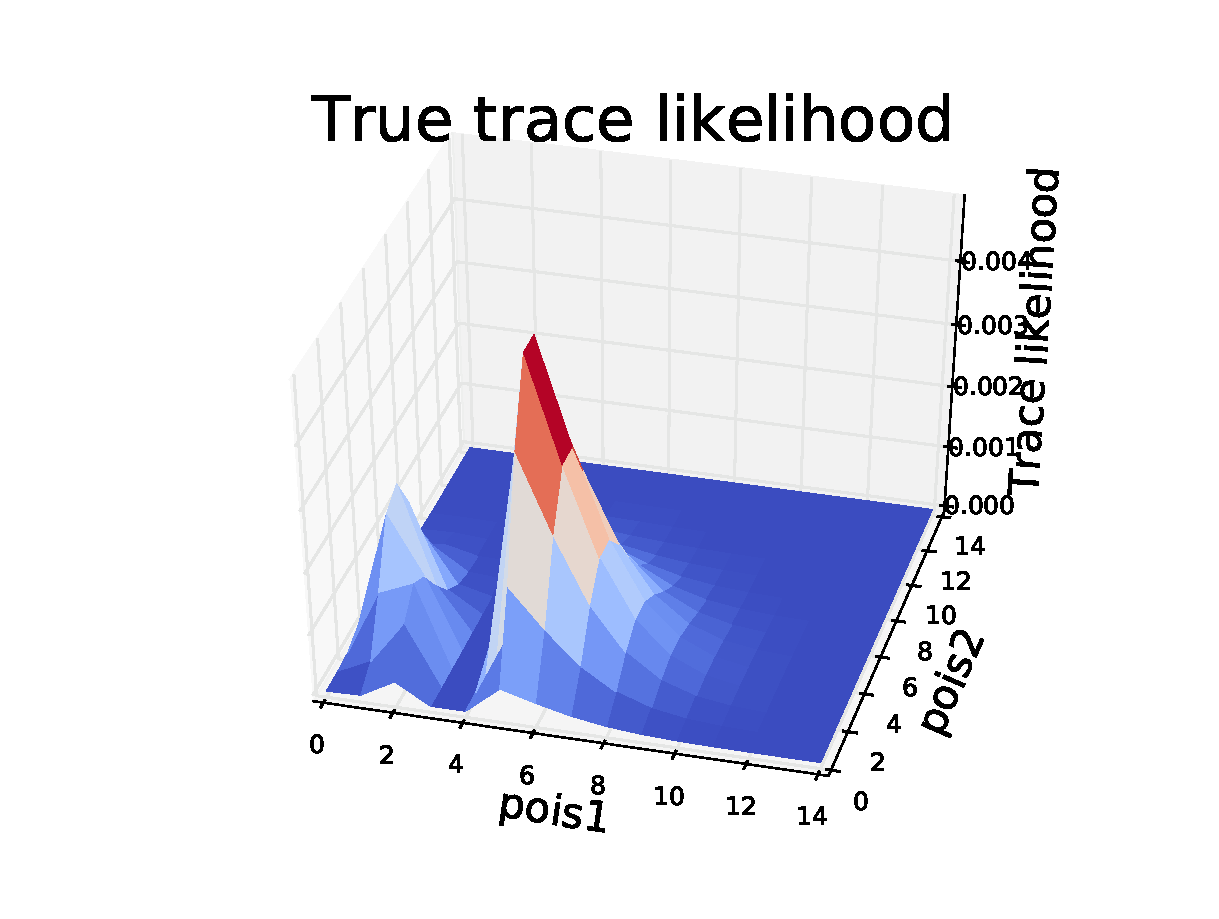
\includegraphics[width=\textwidth]{BranchTraceLik}
                \caption{Space of trace likelihoods if both variables are always sampled.}
                \label{fig:branchTraceLik}
        \end{subfigure}
        ~ 
        \begin{subfigure}[b]{0.48\textwidth}
                \centering
                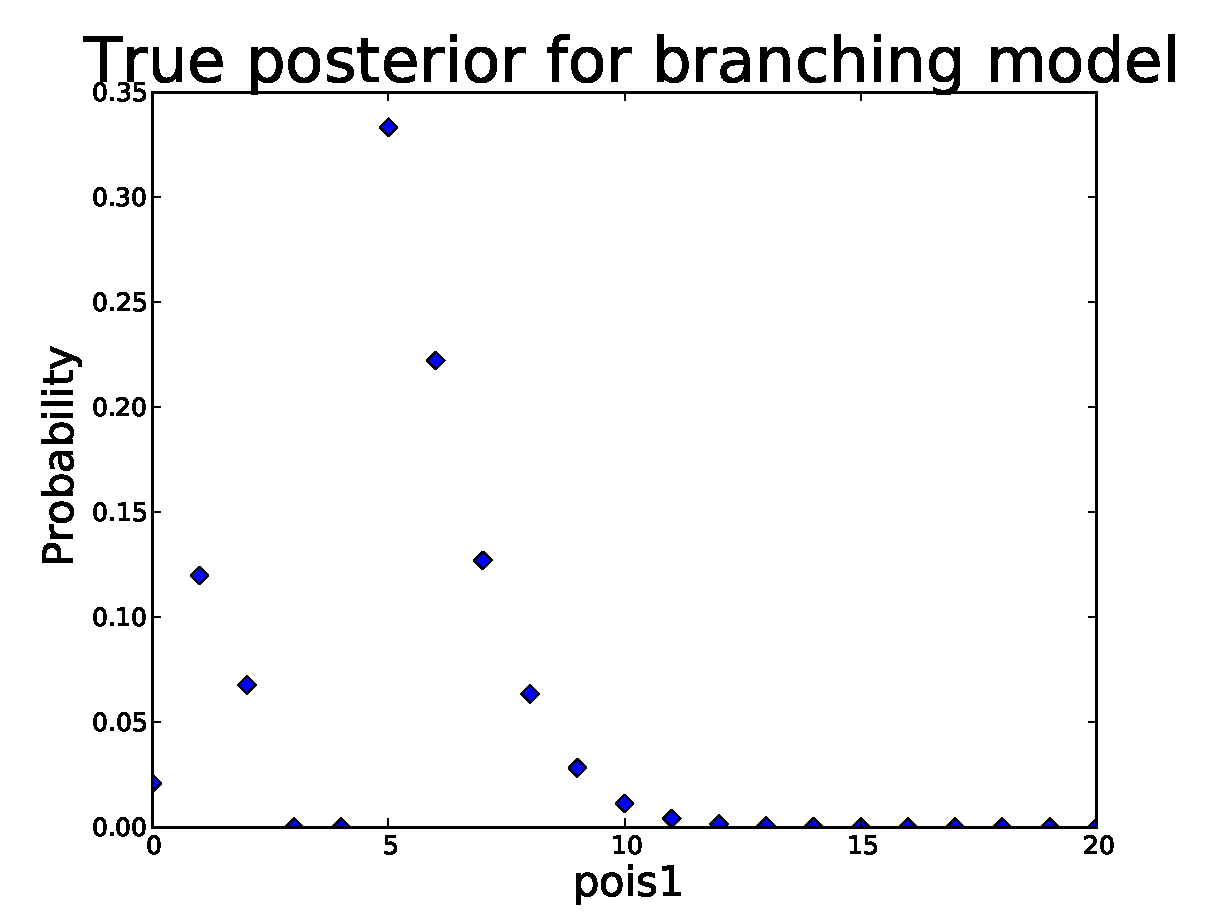
\includegraphics[width=\textwidth]{BranchPost}
                \caption{True posterior of Branching model.}
                \label{fig:branchPost}
        \end{subfigure}
\end{figure}

The issue with trans-dimensional jumps comes from the fact that the naive slice sampling algorithm will not sample the second poisson when it is not necessary, but will still think that the trace likelihoods between runs with different numbers of sampled variables are comparable. In doing so, the slice sampler will be pretending to be sampling from a 2D trace likelihood even when it really is 1D. The space of likelihoods implied by the naive slice sampling implementation is shown in Figure \ref{fig:branchWrongTraceLik}. Integrating out the pois2 variable from this incorrect likelihood space results in the implied posterior shown in Figrue \ref{fig:branchWrongPost}. This wrong posterior is the one which naive slice sampling will be attempting to infer.

\begin{figure}[h]
        \centering
        \begin{subfigure}[b]{0.48\textwidth}
                \centering
                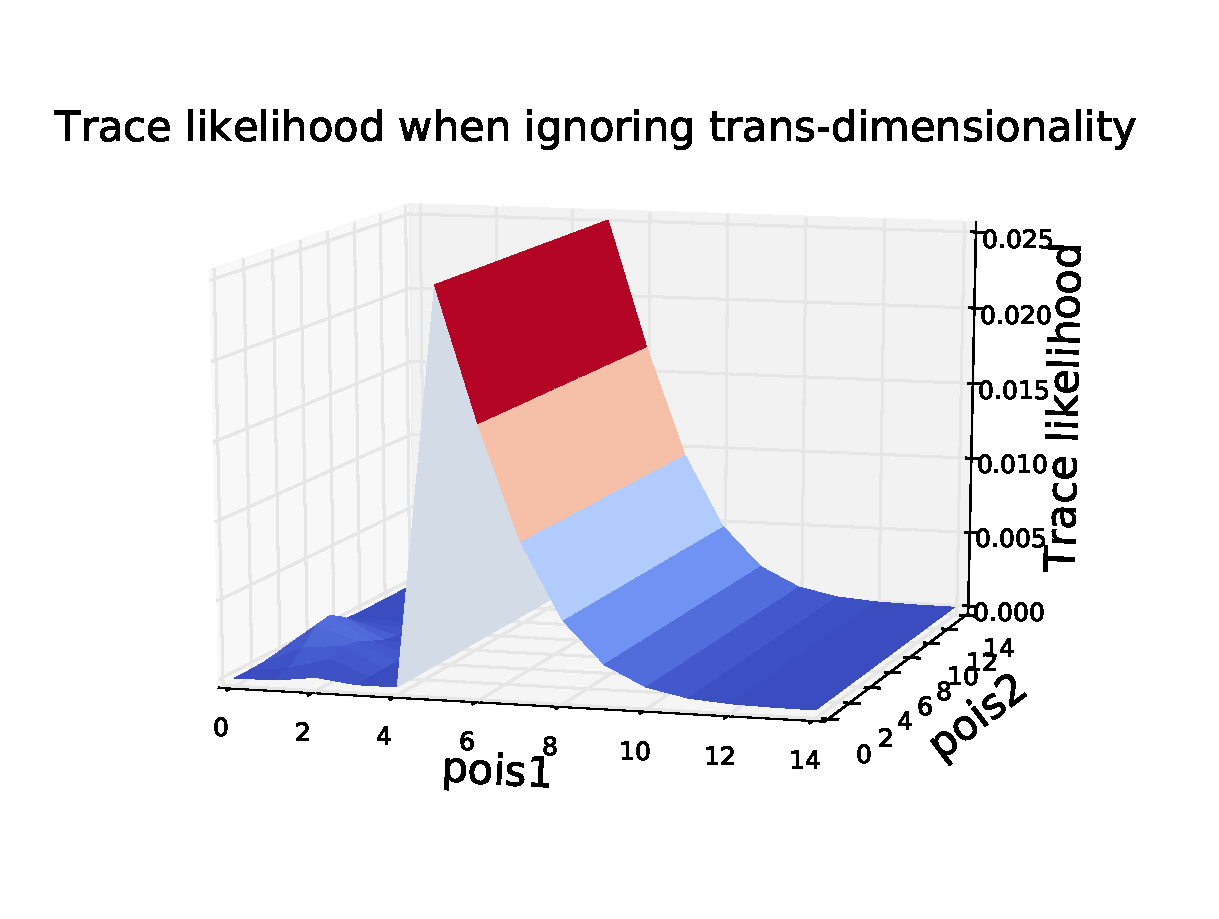
\includegraphics[width=\textwidth]{BranchWrongTraceLik}
                \caption{Space of trace likelihoods if both variables are always sampled.}
                \label{fig:branchWrongTraceLik}
        \end{subfigure}
        ~ 
        \begin{subfigure}[b]{0.48\textwidth}
                \centering
                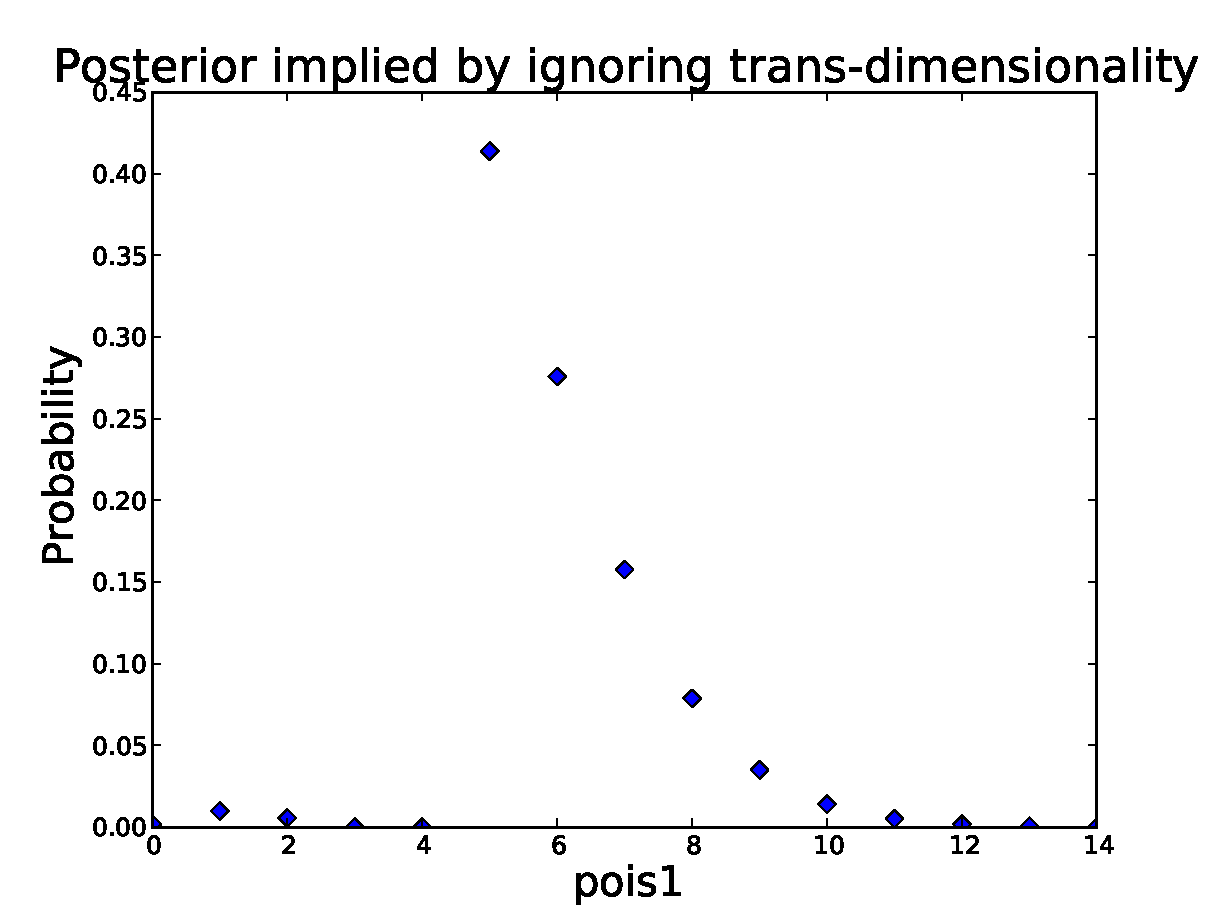
\includegraphics[width=\textwidth]{BranchWrongPost}
                \caption{Space of trace likelihoods implied by naive slice sampling.}
                \label{fig:branchWrongPost}
        \end{subfigure}
\end{figure}

Next we'll look at one simple attempt to correct for trans-dimensional jumps, by thinking in terms of fresh and stale likelihoods, as in the metropolis acceptance ratio. We define a variable as being stale if it was used in the previous program trace but not in the current one. Conversely, a variable is considered fresh if it is being sampled in the current trace but was not used in the previous one. The correction we propose means that, ehen comparing a trace log-likelihood against the slice's sampled height, we won't simply consider the log likelihood (ll), but instead ll + llStale - llFresh.

This correction means that when we are considering a jump to a lower dimensional space the log-likelihood of the lower dimensional space will be decreased by llStale (i.e. the likelihoods of the variables which are not part of this space). Conversely, when considering a move to a higher dimensional space, the log-likelihood of the higher-dimensional trace will be discounted by llFresh (so only the likelihood of the subset of variables that are also part of the current, lower-dimensional, space count). This simple correction seems to give correct results on the continuous NormalMean3 trans-dimensional model explored above (see Figure \ref{fig:normal4TD}).

\begin{figure}[h]
        \centering
        \begin{subfigure}[b]{0.48\textwidth}
                \centering
                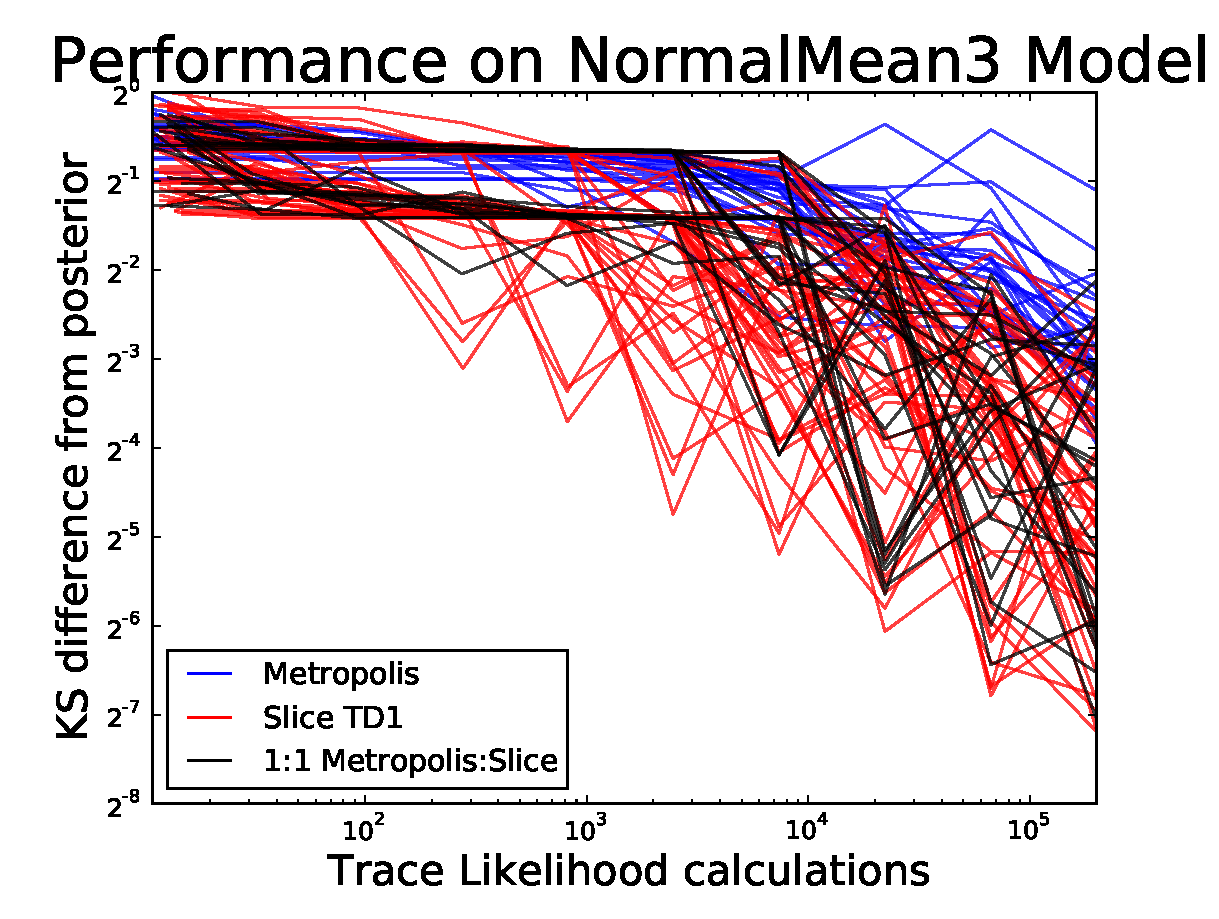
\includegraphics[width=\textwidth]{Normal4TDRuns}
        \end{subfigure}
        ~ 
        \begin{subfigure}[b]{0.48\textwidth}
                \centering
                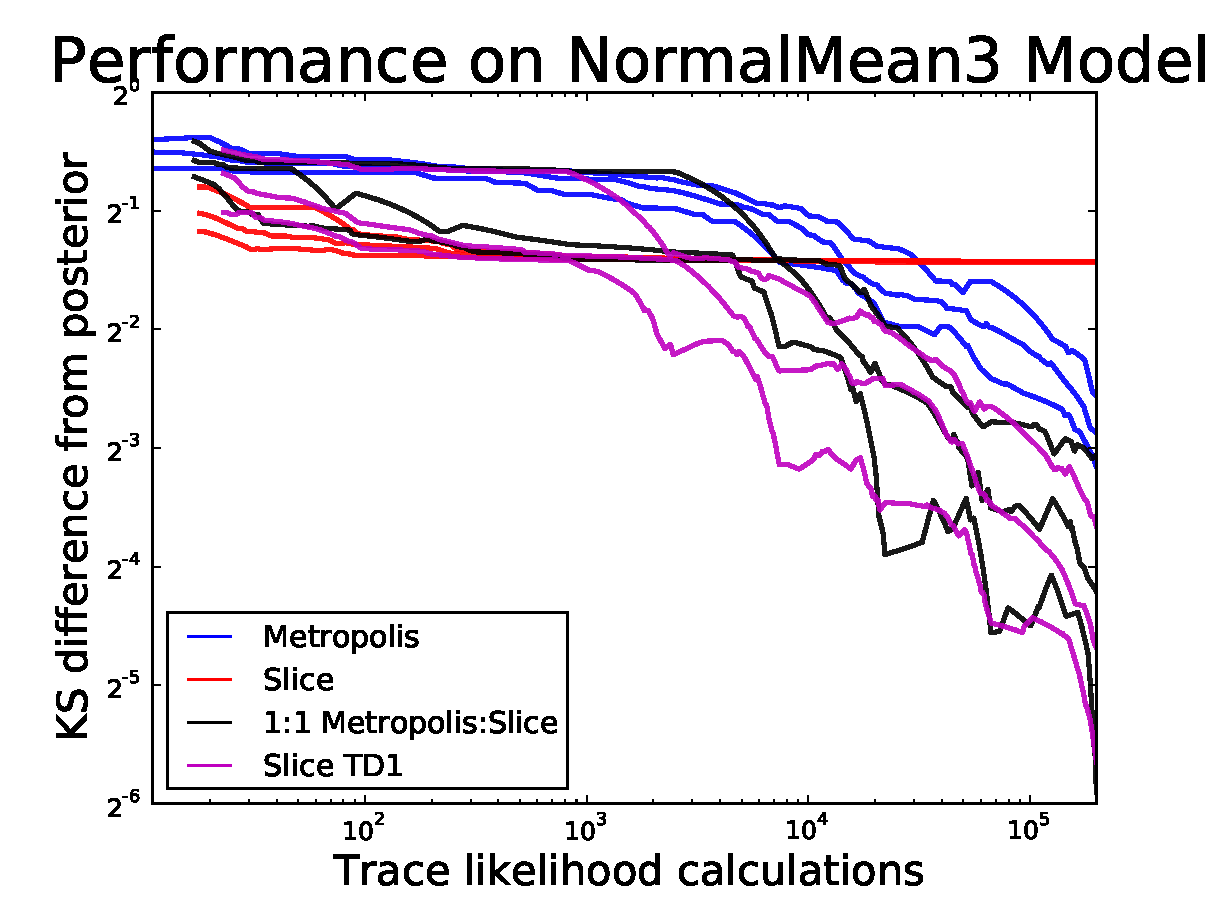
\includegraphics[width=\textwidth]{Normal4TDQuarts}
        \end{subfigure}
    \caption{Runs and quartiles generated by metropolis, a mixture of metropolis and slice, and both the modified and the naive slice algorithms on the NormalMean3 model.}
    \label{fig:normal4TD}
\end{figure}

However, the specification appears to be wrong since it does not converge to the correct distribution on the Branching model (see Figure \ref{fig:branchTD}). Somewhat interestingly, it does seem to converge to a wrong value that's somewhat closer to the true posterior than the naive slice sampling does.

\begin{figure}[h]
        \centering
        \begin{subfigure}[b]{0.48\textwidth}
                \centering
                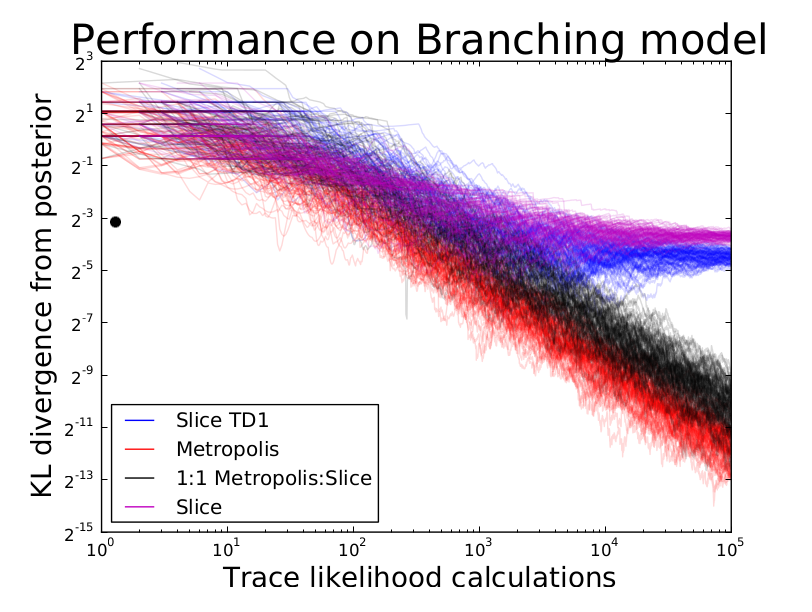
\includegraphics[width=\textwidth]{BranchTDRuns}
        \end{subfigure}
        ~ 
        \begin{subfigure}[b]{0.48\textwidth}
                \centering
                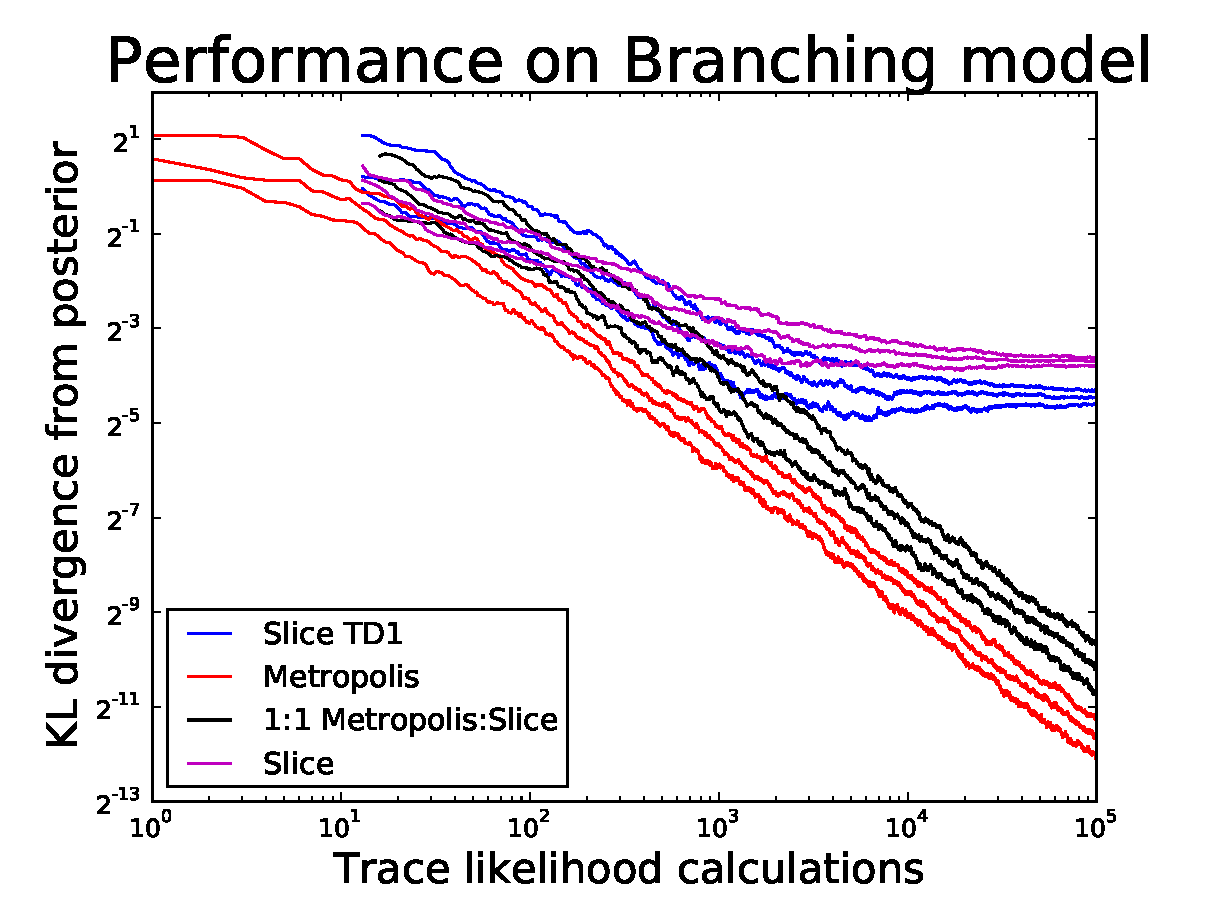
\includegraphics[width=\textwidth]{BranchTDQuarts}
        \end{subfigure}
    \caption{Runs and quartiles generated by metropolis, a mixture of metropolis and slice, and both the corrected slice and the naive slice algorithms on the Branching model.}
    \label{fig:branchTD}
\end{figure}

\section{Quasi-Monte Carlo}
Another possible improvement on naive MC is, rather than sampling randomly from the unit interval, to instead make use of a low-discrepancy sequence that will tend to cover the interval faster \cite{robert2004monte}.

A simple sequence we can use in the 1-dimensional case is the Van der Corput sequence.
We test the performance of this sequence by considering time to mode of neighbourhood for a interval of size 100, neighbourhood of size 1 and modes in the range $[0.5, 1.5, \ldots 99.5]$
Naive metropolis will find this neighbourhood, on average in 100 steps. Using the Van der Corput sequence reduces this to 56 samples. 

The slice sampling technique explored above, however,  managed reductions to 10 and 20 steps respectively (depending on the likelihood function). Therefore I choose to focus on developing the slice sampling technique rather than further investigation Quasi-Monte Carlo methods.


